
\documentclass[10pt,a4paper]{article}
\usepackage[a4paper,margin=14mm,top=18mm,bottom=20mm,headheight=12pt,headsep=5mm,footskip=9mm]{geometry}
\usepackage{fontspec}
\usepackage{xcolor}
\usepackage{graphicx}
\usepackage{tikz}
\usepackage{eso-pic}
\usepackage{tabularx}
\usepackage{array}
\usepackage{fancyhdr}
\usepackage{needspace}
\usepackage{multicol}
\usepackage{enumitem}
\defaultfontfeatures{Ligatures=NoCommon}
\IfFontExistsTF{Noto Sans CJK SC}{\setmainfont{Noto Sans CJK SC}\setsansfont{Noto Sans CJK SC}}{\setmainfont{DejaVu Sans}\setsansfont{DejaVu Sans}}
\IfFontExistsTF{DejaVu Sans}{\newfontfamily\BOQuoteFont{DejaVu Sans}}{\newfontfamily\BOQuoteFont{Latin Modern Sans}}
\newcommand{\BOApos}{{\BOQuoteFont\char"0027}}
\definecolor{BOBlue}{HTML}{0E6B72}
\definecolor{BOBright}{HTML}{20A66A}
\definecolor{BOGreen}{HTML}{00A651}
\definecolor{BONavy}{HTML}{1B2A34}
\definecolor{BOText}{HTML}{24323A}
\definecolor{BOMuted}{HTML}{7C878E}
\definecolor{BOLine}{HTML}{D9E1E6}
\definecolor{BOLight}{HTML}{F2F6F4}
\setlength{\parindent}{0pt}
\setlength{\parskip}{3.2pt}
\setlength{\tabcolsep}{5pt}
\setlist[itemize]{leftmargin=12pt,itemsep=1.5pt,topsep=2pt,parsep=0pt}
\renewcommand{\arraystretch}{1.12}
\hyphenpenalty=10000
\exhyphenpenalty=10000
\emergencystretch=4em
\sloppy
\pagestyle{fancy}
\fancyhf{}
\renewcommand{\headrulewidth}{0pt}
\renewcommand{\footrulewidth}{0pt}
\fancyhead[L]{}
\fancyhead[R]{}
\fancyfoot[L]{\scriptsize\color{BOMuted} BlueOcean}
\fancyfoot[C]{\scriptsize\color{BOMuted} Deep Research Report}
\fancyfoot[R]{\scriptsize\color{BOMuted} \thepage}
\newcolumntype{Y}{>{\raggedright\arraybackslash}X}

\begin{document}
\raggedright

\clearpage
\thispagestyle{empty}
\AddToShipoutPictureBG*{\AtPageLowerLeft{
\includegraphics[width=\paperwidth,height=\paperheight]{assets/cover-ai.png}}}

\vspace*{7mm}
\noindent\hspace*{2mm}{\setlength{\fboxsep}{7mm}\fcolorbox{white}{white}{\begin{minipage}{118mm}
{\sffamily\scriptsize\bfseries\color{BOMuted} BLUEOCEAN RESEARCH}\par\vspace{5pt}
{\textcolor{BOGreen}{\rule{118mm}{1.5pt}}}\par\vspace{8pt}
{\sffamily\fontsize{24}{29}\selectfont\color{BONavy} Nuclear Fusion Commercialization Outlook and Strategic Implications}\par\vspace{10pt}
{\sffamily\scriptsize\bfseries\color{BOText} Nuclear fusion commercialization outlook and strategic implications}\par\vspace{3pt}
{\sffamily\scriptsize\color{BOMuted} 2026-06-03}
\end{minipage}}}
\vfill
\begin{flushright}
{\sffamily\bfseries\Large\color{white} BlueOcean}\hspace*{3mm}
\end{flushright}
\vspace*{7mm}
\clearpage

\clearpage
\noindent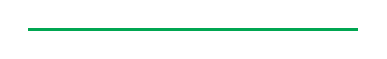
\begin{tikzpicture}
\fill[BOGreen] (0,0) rectangle (42mm,1.2pt);
\end{tikzpicture}\par\vspace{8pt}
{\sffamily\fontsize{26}{31}\selectfont\color{BONavy} Contents}\par\vspace{10pt}
\begin{minipage}[t]{0.57\linewidth}
\begin{tabularx}{\linewidth}{p{12mm}Y}
\textcolor{BOGreen}{\bfseries 03} & {\footnotesize Fusion commercialization timelines have shortened but remain uncertain} \\[4pt]
\textcolor{BOGreen}{\bfseries 04} & {\footnotesize Proof, economics and timing determine whether fusion changes capital allocation} \\[4pt]
\textcolor{BOGreen}{\bfseries 05} & {\footnotesize Decision readiness still depends on verified proof points} \\[4pt]
\textcolor{BOGreen}{\bfseries 07} & {\footnotesize Fusion Commercialization Timelines Are Accelerating but Remain Uncertain} \\[4pt]
\textcolor{BOGreen}{\bfseries 09} & {\footnotesize Fusion Economics: High Initial Costs but Potential for Long-Term Competitiveness} \\[4pt]
\textcolor{BOGreen}{\bfseries 11} & {\footnotesize Global Fusion Investment Surge: Opportunities and Risks} \\[4pt]
\textcolor{BOGreen}{\bfseries 12} & {\footnotesize Geopolitical Implications: Energy Security, Proliferation, and Strategic Competition} \\[4pt]
\textcolor{BOGreen}{\bfseries 14} & {\footnotesize Regulatory and Public Acceptance: Building the Framework for Fusion Deployment} \\[4pt]
\textcolor{BOGreen}{\bfseries 15} & {\footnotesize Technical Hurdles: The Path to Commercial Fusion} \\[4pt]
\textcolor{BOGreen}{\bfseries 17} & {\footnotesize Nuclear Fusion Commercialization Outlook and Strategic Implications should be managed as a staged strategic option, not a binary bet} \\[4pt]
\textcolor{BOGreen}{\bfseries 18} & {\footnotesize Commercial readiness depends on bankability, deliverability and repeat customer proof} \\[4pt]
\textcolor{BOGreen}{\bfseries 20} & {\footnotesize About the research} \\[4pt]
\end{tabularx}
\end{minipage}\hfill\begin{minipage}[t]{0.36\linewidth}
\fcolorbox{BOLine}{BOLight}{\begin{minipage}{0.91\linewidth}\vspace{5pt}
{\textcolor{BOGreen}{\scriptsize\bfseries SENIOR-LEADERSHIP QUESTIONS}}\par\vspace{5pt}
\begin{tabularx}{\linewidth}{p{8mm}Y}
\textcolor{BOGreen}{\bfseries 01} & {\scriptsize Fusion commercialization timelines have shortened but remain uncertain; first power plants likely between 2035 and 2050. The next five years are critical: if key} \\[6pt]
\textcolor{BOGreen}{\bfseries 02} & {\scriptsize Fusion\BOApos{}s levelized cost of energy (LCOE) is projected at \$50-100/MWh by 2050, competitive with fission and natural gas with carbon capture, but higher than solar} \\[6pt]
\textcolor{BOGreen}{\bfseries 03} & {\scriptsize Global fusion investment has surged, with private funding exceeding \$6 billion cumulatively by 2025, driven by breakthroughs like LLNL\BOApos{}s ignition. However, investment} \\[6pt]
\textcolor{BOGreen}{\bfseries 04} & {\scriptsize Geopolitical implications are significant: fusion could reduce energy import dependence but also create new proliferation risks. Nations with fusion leadership (US} \\[6pt]
\end{tabularx}\vspace{4pt}
{\scriptsize\color{BOMuted} The report uses 14 exhibits across Bar, bubble, line, matrix, stacked bar to keep the narrative anchored in comparable facts.}\par\vspace{5pt}
\end{minipage}}
\end{minipage}
\clearpage

\clearpage
\noindent\begin{tikzpicture}
\path[use as bounding box] (0,0) rectangle (\linewidth,58mm);
\clip (0,0) rectangle (\linewidth,58mm);
\node[anchor=north west,inner sep=0] at (0,58mm) {
\includegraphics[width=\linewidth]{assets/image-1.png}};
\end{tikzpicture}
\vspace{0pt}
\noindent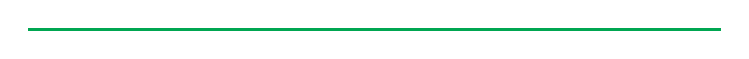
\begin{tikzpicture}
\fill[BOGreen] (0,0) rectangle (88mm,1.2pt);
\end{tikzpicture}\par\vspace{8pt}
{\sffamily\fontsize{24}{30}\selectfont\color{BONavy} Fusion commercialization timelines have shortened but remain uncertain}\par\vspace{11pt}
\begin{minipage}[t]{0.44\linewidth}
{\sffamily\fontsize{17}{23}\selectfont\color{BOGreen} Fusion commercialization timelines have shortened but remain uncertain}\par\vspace{10pt}
{\small\color{BOText} Nuclear fusion is approaching a pivotal inflection point: after decades of scientific progress, private and public investments are accelerating, with first commercial plants potentially online by the mid-2030s. However, significant technical, economic, and regulatory hurdles remain, and fusion\BOApos{}s ultimate competitiveness will depend on cost trajectories relative to rapidly improving renewables and storage. For senior executives, the strategic imperative is to monitor fusion developments closely, invest selectively in enabling technologies and partnerships, and prepare for a gradual adoption scenario that could reshape energy markets, geopolitics, and investment portfolios over the next two decades. The key decision is whether to commit capital now for long-term positioning or wait for clearer proof points, balancing the risk of missing early-mover advantages against the risk of premature investment.}\par
\end{minipage}\hfill\begin{minipage}[t]{0.45\linewidth}
{\small\color{BOText} Fusion\BOApos{}s levelized cost of energy (LCOE) is projected at \$50-100/MWh by 2050, competitive with fission and natural gas with carbon capture, but higher than solar and wind. Its value proposition is baseload reliability and complementarity with intermittent renewables. Global fusion investment has surged, with private funding exceeding \$6 billion cumulatively by 2025, driven by breakthroughs like LLNL\BOApos{}s ignition. However, investment remains concentrated in a few ventures; due diligence on technology readiness is critical. Geopolitical implications are significant: fusion could reduce energy import dependence but also create new proliferation risks. Nations with fusion leadership (US, China, EU) will gain energy security and export opportunities.}\par
\end{minipage}

\clearpage
\noindent\begin{tikzpicture}
\path[use as bounding box] (0,0) rectangle (\linewidth,62mm);
\clip (0,0) rectangle (\linewidth,62mm);
\node[anchor=north west,inner sep=0] at (0,62mm) {
\includegraphics[width=\linewidth]{assets/image-2.png}};
\end{tikzpicture}
\vspace{0pt}
\noindent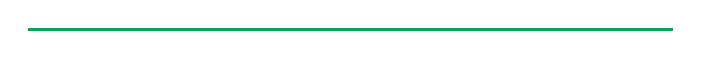
\begin{tikzpicture}
\fill[BOGreen] (0,0) rectangle (82mm,1.2pt);
\end{tikzpicture}\par\vspace{8pt}
{\sffamily\fontsize{23}{29}\selectfont\color{BONavy} Fusion Commercialization Timelines Are Accelerating but Remain Uncertain}\par\vspace{8pt}
{\sffamily\fontsize{16}{21}\selectfont\color{BOGreen} Fusion is no longer a distant dream but a credible technology with a defined-if uncertain-path to commercialization; the next five years will be critical.}\par\vspace{9pt}
\begin{minipage}[t]{0.46\linewidth}
{\small Fusion commercialization timelines have shortened but remain uncertain; first power plants likely between 2035 and 2050. Private ventures like Commonwealth Fusion Systems target 2035 for SPARC, while ITER\BOApos{}s first plasma is delayed to 2035. DOE milestone program aims for pilot plant by 2030s. National Academies study notes 2040-2050 as realistic for grid-scale fusion. Do not expect fusion to impact energy markets before 2035, but early technology validation could create strategic value for first movers in supply}\par
{\small Global fusion investment has surged, with private funding exceeding \$6 billion cumulatively by 2025, driven by breakthroughs like LLNL\BOApos{}s ignition. Fusion Industry Association 2024 report shows private fusion investment grew from \$300 million in 2020 to over \$6 billion total by 2025. LLNL\BOApos{}s 2022 ignition milestone (2.15 MJ output) catalyzed investor interest. DOE\BOApos{}s milestone program allocates \$50 million to private-public partnerships. The influx of private capital signals growing confidence, but investment remains}\par
\end{minipage}\hfill\begin{minipage}[t]{0.46\linewidth}
{\small Fusion\BOApos{}s levelized cost of energy (LCOE) is projected to be \$50-100/MWh by 2050, competitive with fission and baseload renewables but higher than solar and wind. Fusion Industry Association reports estimate LCOE of \$50-100/MWh for first-of-a-kind plants, declining with learning. DOE and IAEA analyses suggest fusion will be cost-competitive with nuclear fission and natural gas with carbon capture, but not with solar PV at \$20-30/MWh. Fusion is unlikely to disrupt low-cost solar and wind markets; its value}\par
{\small Geopolitical implications are significant: fusion could reduce energy import dependence, but also create new proliferation risks and shift strategic advantages. IAEA notes fusion fuel (deuterium, tritium) is widely available, but tritium breeding technology is unproven. China\BOApos{}s aggressive fusion program (ITER participation, domestic projects) could leapfrog Western efforts. DOE and National Academies highlight non-proliferation concerns from fusion neutron sources. Nations with fusion leadership (US, China, EU)}\par
\end{minipage}

\clearpage
{\textcolor{BOGreen}{\scriptsize\bfseries EXHIBIT 1}}\par\vspace{4pt}
{\sffamily\fontsize{17}{21}\selectfont\color{BONavy} Decision readiness still depends on verified proof points}\par
{\small\color{BOText} Customer, cost and partner proof remain the main underwriting gaps for Nuclear Fusion Commercialization Outlook and Strategic Implications}\par\vspace{6pt}
\noindent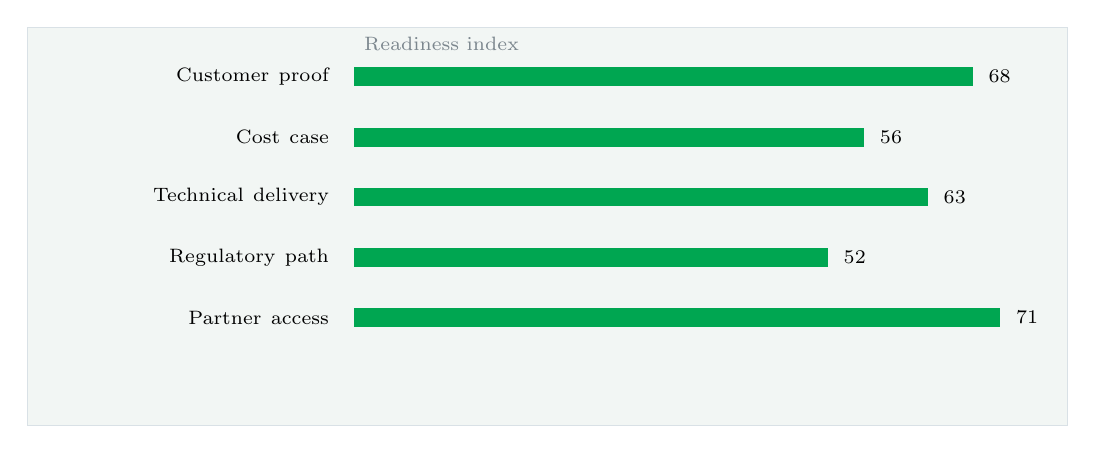
\begin{tikzpicture}[x=1cm,y=1cm]
\path[use as bounding box] (0,0) rectangle (13.20,5.05);
\fill[BOLight] (0,0) rectangle (13.20,5.05);
\draw[BOLine,line width=.35pt] (0,0) rectangle (13.20,5.05);
\node[anchor=west] at (4.15,4.85) {\scriptsize\color{BOMuted} Readiness index};
\node[anchor=east,align=right,text width=3.93cm] at (3.95,4.43) {\scriptsize Customer proof};
\fill[BOLight] (4.15,4.31) rectangle (12.35,4.55);
\fill[BOGreen] (4.15,4.31) rectangle (12.00,4.55);
\node[anchor=west] at (12.08,4.43) {\scriptsize 68};
\node[anchor=east,align=right,text width=3.93cm] at (3.95,3.66) {\scriptsize Cost case};
\fill[BOLight] (4.15,3.54) rectangle (12.35,3.78);
\fill[BOGreen] (4.15,3.54) rectangle (10.62,3.78);
\node[anchor=west] at (10.70,3.66) {\scriptsize 56};
\node[anchor=east,align=right,text width=3.93cm] at (3.95,2.90) {\scriptsize Technical delivery};
\fill[BOLight] (4.15,2.78) rectangle (12.35,3.02);
\fill[BOGreen] (4.15,2.78) rectangle (11.43,3.02);
\node[anchor=west] at (11.51,2.90) {\scriptsize 63};
\node[anchor=east,align=right,text width=3.93cm] at (3.95,2.13) {\scriptsize Regulatory path};
\fill[BOLight] (4.15,2.01) rectangle (12.35,2.25);
\fill[BOGreen] (4.15,2.01) rectangle (10.16,2.25);
\node[anchor=west] at (10.24,2.13) {\scriptsize 52};
\node[anchor=east,align=right,text width=3.93cm] at (3.95,1.37) {\scriptsize Partner access};
\fill[BOLight] (4.15,1.25) rectangle (12.35,1.49);
\fill[BOGreen] (4.15,1.25) rectangle (12.35,1.49);
\node[anchor=west] at (12.43,1.37) {\scriptsize 71};
\end{tikzpicture}\par\vspace{2pt}
\vspace{1pt}\noindent\begin{minipage}[t]{0.56\linewidth}
{\footnotesize\color{BOText} The exhibit ranks the proof points a CEO should ask teams to close before moving from monitoring to commitment.}\par
\end{minipage}\hfill\begin{minipage}[t]{0.36\linewidth}
{\scriptsize\color{BOText}\begin{tabular}{p{31mm}>{\raggedleft\arraybackslash}p{18mm}}
\multicolumn{2}{l}{\textcolor{BOGreen}{\bfseries Visible readout}}\\[2pt]
Customer proof & \textbf{68}\\[1pt]
Cost case & \textbf{56}\\[1pt]
Technical delivery & \textbf{63}\\[1pt]
Regulatory path & \textbf{52}\\[1pt]
Partner access & \textbf{71}\\[1pt]
\end{tabular}}\par
\end{minipage}\par\vspace{1pt}
\vspace{4pt}{\footnotesize\color{BOText} The exhibit ranks the proof points a CEO should ask teams to close before moving from monitoring to commitment.}\par
{\scriptsize\color{BOMuted} BlueOcean public-source synthesis.}\par
\vspace{9pt}\textcolor{BOLine}{\rule{\linewidth}{0.3pt}}\vspace{8pt}
{\textcolor{BOGreen}{\scriptsize\bfseries EXHIBIT 2}}\par\vspace{4pt}
{\sffamily\fontsize{17}{21}\selectfont\color{BONavy} Commitment posture should shift as proof matures}\par
{\small\color{BOText} Resource posture for Nuclear Fusion Commercialization Outlook and Strategic Implications}\par\vspace{6pt}
\noindent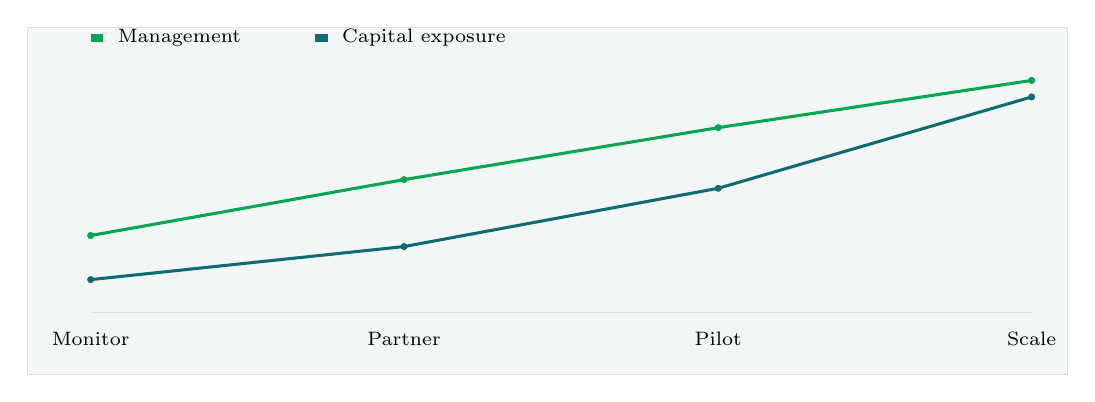
\begin{tikzpicture}[x=1cm,y=1cm]
\path[use as bounding box] (0,0) rectangle (13.20,4.40);
\fill[BOLight] (0,0) rectangle (13.20,4.40);
\draw[BOLine,line width=.35pt] (0,0) rectangle (13.20,4.40);
\draw[BOLine] (0.80,0.78) -- (12.75,0.78);
\draw[BOGreen,line width=1.1pt] (0.80,1.76) -- (4.78,2.47) -- (8.77,3.13) -- (12.75,3.73);
\fill[BOGreen] (0.80,1.76) circle (.045);
\fill[BOGreen] (4.78,2.47) circle (.045);
\fill[BOGreen] (8.77,3.13) circle (.045);
\fill[BOGreen] (12.75,3.73) circle (.045);
\draw[BOBlue,line width=1.1pt] (0.80,1.20) -- (4.78,1.62) -- (8.77,2.36) -- (12.75,3.52);
\fill[BOBlue] (0.80,1.20) circle (.045);
\fill[BOBlue] (4.78,1.62) circle (.045);
\fill[BOBlue] (8.77,2.36) circle (.045);
\fill[BOBlue] (12.75,3.52) circle (.045);
\node[anchor=north,align=center,text width=1.8cm] at (0.80,0.66) {\scriptsize Monitor};
\node[anchor=north,align=center,text width=1.8cm] at (4.78,0.66) {\scriptsize Partner};
\node[anchor=north,align=center,text width=1.8cm] at (8.77,0.66) {\scriptsize Pilot};
\node[anchor=north,align=center,text width=1.8cm] at (12.75,0.66) {\scriptsize Scale};
\fill[BOGreen] (0.80,4.22) rectangle (0.96,4.32);
\node[anchor=west] at (1.02,4.27) {\scriptsize Management};
\fill[BOBlue] (3.65,4.22) rectangle (3.81,4.32);
\node[anchor=west] at (3.87,4.27) {\scriptsize Capital exposure};
\end{tikzpicture}\par\vspace{2pt}
\vspace{1pt}\noindent\begin{minipage}[t]{0.56\linewidth}
{\footnotesize\color{BOText} Capital exposure should lag evidence maturity rather than lead it.}\par
\end{minipage}\hfill\begin{minipage}[t]{0.36\linewidth}
{\scriptsize\color{BOText}\begin{tabular}{p{31mm}>{\raggedleft\arraybackslash}p{18mm}}
\multicolumn{2}{l}{\textcolor{BOGreen}{\bfseries Visible readout}}\\[2pt]
Monitor & \textbf{40}\\[1pt]
Partner & \textbf{72}\\[1pt]
Pilot & \textbf{112}\\[1pt]
Scale & \textbf{162}\\[1pt]
\end{tabular}}\par
\end{minipage}\par\vspace{1pt}
\vspace{4pt}{\footnotesize\color{BOText} Capital exposure should lag evidence maturity rather than lead it.}\par
{\scriptsize\color{BOMuted} BlueOcean scenario synthesis.}\par

\clearpage
{\textcolor{BOGreen}{\scriptsize\bfseries EXHIBIT 3}}\par\vspace{4pt}
{\sffamily\fontsize{17}{21}\selectfont\color{BONavy} Key risks should be ranked by severity and manageability}\par
{\small\color{BOText} Risk exposure for Nuclear Fusion Commercialization Outlook and Strategic Implications}\par\vspace{6pt}
\noindent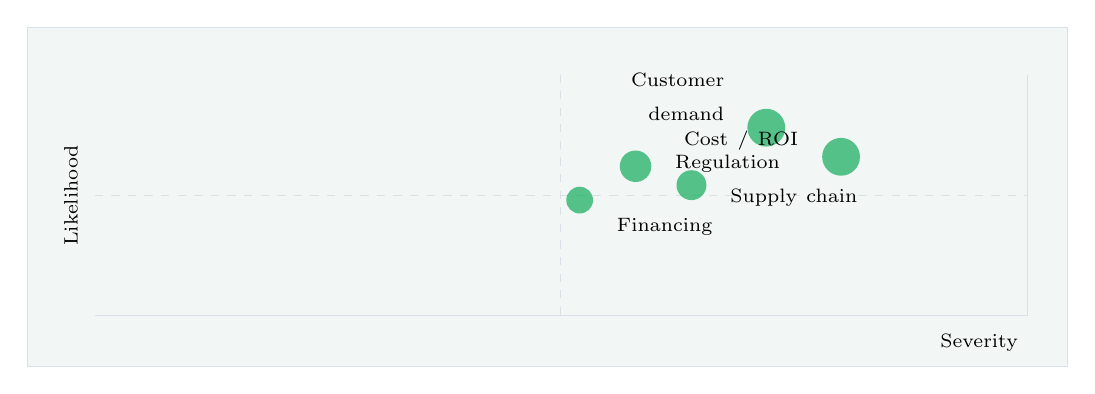
\begin{tikzpicture}[x=1cm,y=1cm]
\path[use as bounding box] (0,0) rectangle (13.20,4.30);
\fill[BOLight] (0,0) rectangle (13.20,4.30);
\draw[BOLine,line width=.35pt] (0,0) rectangle (13.20,4.30);
\draw[BOLine] (0.85,0.65) -- (12.70,0.65) -- (12.70,3.70);
\draw[BOLine,dashed] (0.85,2.17) -- (12.70,2.17);
\draw[BOLine,dashed] (6.77,0.65) -- (6.77,3.70);
\fill[BOGreen,opacity=.65] (9.38,3.03) circle (0.24);
\node[anchor=east,align=right,text width=2.10cm] at (8.97,3.42) {\scriptsize Customer demand};
\fill[BOGreen,opacity=.65] (10.33,2.66) circle (0.24);
\node[anchor=east,align=right,text width=2.10cm] at (9.91,2.87) {\scriptsize Cost / ROI};
\fill[BOGreen,opacity=.65] (7.72,2.54) circle (0.20);
\node[anchor=west,align=left,text width=2.10cm] at (8.10,2.57) {\scriptsize Regulation};
\fill[BOGreen,opacity=.65] (8.43,2.30) circle (0.19);
\node[anchor=west,align=left,text width=2.10cm] at (8.80,2.14) {\scriptsize Supply chain};
\fill[BOGreen,opacity=.65] (7.01,2.11) circle (0.17);
\node[anchor=west,align=left,text width=2.10cm] at (7.36,1.77) {\scriptsize Financing};
\node[anchor=north east] at (12.70,0.53) {\scriptsize Severity};
\node[anchor=center,rotate=90] at (0.55,2.17) {\scriptsize Likelihood};
\end{tikzpicture}\par\vspace{2pt}
\vspace{1pt}\noindent\begin{minipage}[t]{0.56\linewidth}
{\footnotesize\color{BOText} Bubble size indicates the management attention required.}\par
\end{minipage}\hfill\begin{minipage}[t]{0.36\linewidth}
{\scriptsize\color{BOText}\begin{tabular}{p{31mm}>{\raggedleft\arraybackslash}p{18mm}}
\multicolumn{2}{l}{\textcolor{BOGreen}{\bfseries Position}}\\[2pt]
Customer demand & \textbf{72 / 78}\\[1pt]
Cost / ROI & \textbf{80 / 66}\\[1pt]
Regulation & \textbf{58 / 62}\\[1pt]
Supply chain & \textbf{64 / 54}\\[1pt]
Financing & \textbf{52 / 48}\\[1pt]
\end{tabular}}\par
\end{minipage}\par\vspace{1pt}
\vspace{4pt}{\footnotesize\color{BOText} Bubble size indicates the management attention required.}\par
{\scriptsize\color{BOMuted} BlueOcean risk screen.}\par
\vspace{9pt}\textcolor{BOLine}{\rule{\linewidth}{0.3pt}}\vspace{8pt}
{\textcolor{BOGreen}{\scriptsize\bfseries EXHIBIT 4}}\par\vspace{4pt}
{\sffamily\fontsize{17}{21}\selectfont\color{BONavy} Diligence workload concentrates in customer, cost and policy proof}\par
{\small\color{BOText} Near-term validation load for Nuclear Fusion Commercialization Outlook and Strategic Implications}\par\vspace{6pt}
\noindent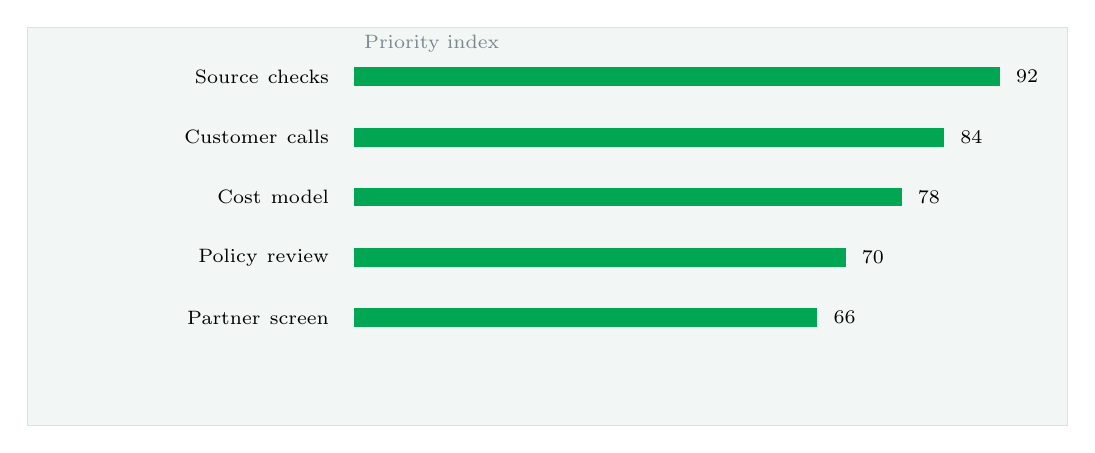
\begin{tikzpicture}[x=1cm,y=1cm]
\path[use as bounding box] (0,0) rectangle (13.20,5.05);
\fill[BOLight] (0,0) rectangle (13.20,5.05);
\draw[BOLine,line width=.35pt] (0,0) rectangle (13.20,5.05);
\node[anchor=west] at (4.15,4.85) {\scriptsize\color{BOMuted} Priority index};
\node[anchor=east,align=right,text width=3.93cm] at (3.95,4.43) {\scriptsize Source checks};
\fill[BOLight] (4.15,4.31) rectangle (12.35,4.55);
\fill[BOGreen] (4.15,4.31) rectangle (12.35,4.55);
\node[anchor=west] at (12.43,4.43) {\scriptsize 92};
\node[anchor=east,align=right,text width=3.93cm] at (3.95,3.66) {\scriptsize Customer calls};
\fill[BOLight] (4.15,3.54) rectangle (12.35,3.78);
\fill[BOGreen] (4.15,3.54) rectangle (11.64,3.78);
\node[anchor=west] at (11.72,3.66) {\scriptsize 84};
\node[anchor=east,align=right,text width=3.93cm] at (3.95,2.90) {\scriptsize Cost model};
\fill[BOLight] (4.15,2.78) rectangle (12.35,3.02);
\fill[BOGreen] (4.15,2.78) rectangle (11.10,3.02);
\node[anchor=west] at (11.18,2.90) {\scriptsize 78};
\node[anchor=east,align=right,text width=3.93cm] at (3.95,2.13) {\scriptsize Policy review};
\fill[BOLight] (4.15,2.01) rectangle (12.35,2.25);
\fill[BOGreen] (4.15,2.01) rectangle (10.39,2.25);
\node[anchor=west] at (10.47,2.13) {\scriptsize 70};
\node[anchor=east,align=right,text width=3.93cm] at (3.95,1.37) {\scriptsize Partner screen};
\fill[BOLight] (4.15,1.25) rectangle (12.35,1.49);
\fill[BOGreen] (4.15,1.25) rectangle (10.03,1.49);
\node[anchor=west] at (10.11,1.37) {\scriptsize 66};
\end{tikzpicture}\par\vspace{2pt}
\vspace{1pt}\noindent\begin{minipage}[t]{0.56\linewidth}
{\footnotesize\color{BOText} The most valuable work closes open questions that can change the decision.}\par
\end{minipage}\hfill\begin{minipage}[t]{0.36\linewidth}
{\scriptsize\color{BOText}\begin{tabular}{p{31mm}>{\raggedleft\arraybackslash}p{18mm}}
\multicolumn{2}{l}{\textcolor{BOGreen}{\bfseries Visible readout}}\\[2pt]
Source checks & \textbf{92}\\[1pt]
Customer calls & \textbf{84}\\[1pt]
Cost model & \textbf{78}\\[1pt]
Policy review & \textbf{70}\\[1pt]
Partner screen & \textbf{66}\\[1pt]
\end{tabular}}\par
\end{minipage}\par\vspace{1pt}
\vspace{4pt}{\footnotesize\color{BOText} The most valuable work closes open questions that can change the decision.}\par
{\scriptsize\color{BOMuted} BlueOcean public-source synthesis.}\par

\clearpage
\label{chap:1}
\noindent\begin{tikzpicture}
\path[use as bounding box] (0,0) rectangle (\linewidth,54mm);
\clip (0,0) rectangle (\linewidth,54mm);
\node[anchor=north west,inner sep=0] at (0,54mm) {
\includegraphics[width=\linewidth]{assets/image-1.png}};
\end{tikzpicture}
\vspace{0pt}
\noindent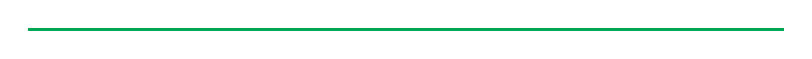
\begin{tikzpicture}
\fill[BOGreen] (0,0) rectangle (96mm,1.2pt);
\end{tikzpicture}\par\vspace{8pt}
{\Large\sffamily\bfseries\color{BONavy} Fusion Commercialization Timelines Are Accelerating but Remain Uncertain}\par\vspace{4pt}
{\sffamily\fontsize{15}{20}\selectfont\color{BOGreen} Fusion is no longer a distant dream but a credible technology with a defined-if uncertain-path to commercialization; the next five years will be critical.}\par\vspace{9pt}
\begin{multicols}{2}
{\small Nuclear fusion has long been considered the \BOApos{}holy grail\BOApos{} of clean energy, but its commercialization has consistently been projected decades away. However, recent developments-including the 2022 ignition milestone at Lawrence Livermore National Laboratory (LLNL) and the rise of well-funded private ventures-have shifted the narrative. The question is no longer whether fusion will work, but when it will become commercially viable and at what cost.}\par
{\small The ITER project, the world\BOApos{}s largest fusion experiment, remains the flagship of international collaboration. Originally scheduled for first plasma in 2020, ITER\BOApos{}s timeline has slipped repeatedly, with the latest estimate targeting 2035 for first plasma and 2040 for full deuterium-tritium operations. ITER is designed to produce 500 MW of fusion power for 400 seconds, demonstrating the physics and engineering of a burning plasma. However, ITER is not a power plant; it will not generate electricity. Its role is to validate the technology for future commercial reactors.}\par
{\small Private fusion companies are pursuing more aggressive timelines. Commonwealth Fusion Systems (CFS), a spinout from MIT, is building SPARC, a compact tokamak using high-temperature superconducting (HTS) magnets. CFS aims to demonstrate net energy gain (Q>10) by 2027 and to have a first commercial plant, ARC, online by the early 2030s. Other notable ventures include TAE Technologies (field-reversed configuration), General Fusion (magnetized target fusion), and Helion Energy (pulsed fusion). Helion has signed a power purchase agreement with Microsoft for 2028, though this timeline is widely viewed as optimistic.}\par
{\small The U.S. Department of Energy (DOE) has launched a Milestone-Based Fusion Development Program, a public-private partnership that provides funding for companies to achieve specific technical milestones. This program aims to accelerate the development of a fusion pilot plant by the 2030s. Similarly, the ARPA-E BETHE program supports innovative fusion concepts that could leapfrog traditional approaches. These initiatives signal strong government commitment but also underscore the technical challenges that remain.}\par
{\small Realistic commercialization timelines vary widely. Optimistic projections from private companies suggest first commercial plants by 2035-2040. More conservative estimates from the National Academies and IAEA point to 2040-2050 for grid-scale fusion. A 2023 report by the Fusion Industry Association found that 25 out of 35 surveyed companies expect to deliver fusion power to the grid by 2035, but this is likely a best-case scenario. The evidence suggests that fusion will not be a significant contributor to global energy supply before 2040, but early movers could gain strategic advantages in technology, supply chains, and site selection.}\par
{\small For leadership teams, the key takeaway is that fusion is no longer a distant dream but a credible technology with a defined-if uncertain-path to commercialization. The next five years will be critical: if SPARC and other demonstrators achieve their milestones, fusion could attract significantly more investment and accelerate timelines. If they fail, the industry may face a \BOApos{}valley of death\BOApos{} that delays commercialization by another decade. Companies should monitor these milestones closely and be prepared to act when proof points are achieved.}\par
\end{multicols}
\label{chap:1:end}

\clearpage
{\textcolor{BOGreen}{\scriptsize\bfseries EXHIBIT 5}}\par\vspace{4pt}
{\sffamily\fontsize{17}{21}\selectfont\color{BONavy} Scenario choices should compare attractiveness with readiness}\par
{\small\color{BOText} Strategic option comparison for Nuclear Fusion Commercialization Outlook and Strategic Implications}\par\vspace{6pt}
\noindent\fcolorbox{BOLine}{BOLight}{\begin{minipage}{0.96\linewidth}\vspace{4pt}{\scriptsize\begin{tabular}{p{38mm}>{\centering\arraybackslash}p{21mm}>{\centering\arraybackslash}p{21mm}>{\centering\arraybackslash}p{21mm}>{\centering\arraybackslash}p{21mm}}
 & {\bfseries Attractiveness} & {\bfseries Readiness} & {\bfseries Confidence} & {\bfseries Capital need} \\
\hline
{\bfseries Fusion Commercialization} & \colorbox{BOGreen}{\textcolor{white}{\strut\hspace{5pt}5\hspace{5pt}}} & \colorbox{BOBlue}{\textcolor{white}{\strut\hspace{5pt}3\hspace{5pt}}} & \colorbox{BOLight}{\textcolor{BOText}{\strut\hspace{5pt}2\hspace{5pt}}} & \colorbox{BOLight}{\textcolor{BOText}{\strut\hspace{5pt}2\hspace{5pt}}} \\
{\bfseries Fusion Economics: High Initial} & \colorbox{BOGreen}{\textcolor{white}{\strut\hspace{5pt}4\hspace{5pt}}} & \colorbox{BOGreen}{\textcolor{white}{\strut\hspace{5pt}4\hspace{5pt}}} & \colorbox{BOBlue}{\textcolor{white}{\strut\hspace{5pt}3\hspace{5pt}}} & \colorbox{BOBlue}{\textcolor{white}{\strut\hspace{5pt}3\hspace{5pt}}} \\
{\bfseries Global Fusion Investment Surge} & \colorbox{BOGreen}{\textcolor{white}{\strut\hspace{5pt}4\hspace{5pt}}} & \colorbox{BOLight}{\textcolor{BOText}{\strut\hspace{5pt}2\hspace{5pt}}} & \colorbox{BOLight}{\textcolor{BOText}{\strut\hspace{5pt}2\hspace{5pt}}} & \colorbox{BOGreen}{\textcolor{white}{\strut\hspace{5pt}4\hspace{5pt}}} \\
{\bfseries Geopolitical Implications} & \colorbox{BOBlue}{\textcolor{white}{\strut\hspace{5pt}3\hspace{5pt}}} & \colorbox{BOBlue}{\textcolor{white}{\strut\hspace{5pt}3\hspace{5pt}}} & \colorbox{BOBlue}{\textcolor{white}{\strut\hspace{5pt}3\hspace{5pt}}} & \colorbox{BOLight}{\textcolor{BOText}{\strut\hspace{5pt}2\hspace{5pt}}} \\
{\bfseries Regulatory and Public} & \colorbox{BOGreen}{\textcolor{white}{\strut\hspace{5pt}5\hspace{5pt}}} & \colorbox{BOBlue}{\textcolor{white}{\strut\hspace{5pt}3\hspace{5pt}}} & \colorbox{BOBlue}{\textcolor{white}{\strut\hspace{5pt}3\hspace{5pt}}} & \colorbox{BOBlue}{\textcolor{white}{\strut\hspace{5pt}3\hspace{5pt}}} \\
\end{tabular}}\vspace{4pt}\end{minipage}}\par\vspace{2pt}
\vspace{1pt}\noindent\begin{minipage}[t]{0.56\linewidth}
{\footnotesize\color{BOText} The matrix ranks where the next validation work should focus.}\par
\end{minipage}\hfill\begin{minipage}[t]{0.36\linewidth}
{\scriptsize\color{BOText}\begin{tabular}{p{31mm}>{\raggedleft\arraybackslash}p{18mm}}
\multicolumn{2}{l}{\textcolor{BOGreen}{\bfseries Matrix readout}}\\[2pt]
Fusion & \textbf{5 / 3}\\[1pt]
Fusion Economics & \textbf{4 / 4}\\[1pt]
Global Fusion & \textbf{4 / 2}\\[1pt]
Geopolitical & \textbf{3 / 3}\\[1pt]
\end{tabular}}\par
\end{minipage}\par\vspace{1pt}
\vspace{4pt}{\footnotesize\color{BOText} The matrix ranks where the next validation work should focus.}\par
{\scriptsize\color{BOMuted} BlueOcean qualitative assessment.}\par
\vspace{9pt}\textcolor{BOLine}{\rule{\linewidth}{0.3pt}}\vspace{8pt}
{\textcolor{BOGreen}{\scriptsize\bfseries EXHIBIT 6}}\par\vspace{4pt}
{\sffamily\fontsize{17}{21}\selectfont\color{BONavy} Validation effort shifts from customer proof to policy and partners}\par
{\small\color{BOText} Quarterly validation mix for Nuclear Fusion Commercialization Outlook and Strategic Implications}\par\vspace{6pt}
\noindent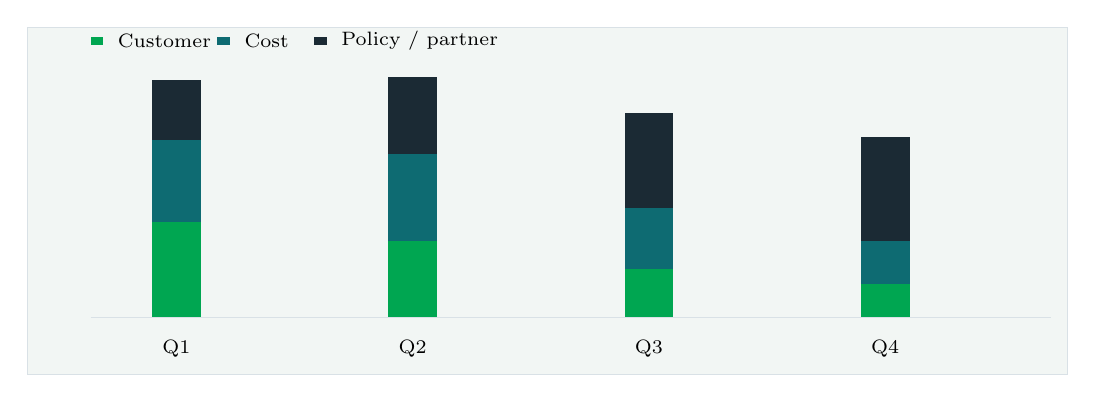
\begin{tikzpicture}[x=1cm,y=1cm]
\path[use as bounding box] (0,0) rectangle (13.20,4.40);
\fill[BOLight] (0,0) rectangle (13.20,4.40);
\draw[BOLine,line width=.35pt] (0,0) rectangle (13.20,4.40);
\draw[BOLine] (0.80,0.72) -- (13.00,0.72);
\fill[BOGreen] (1.58,0.72) rectangle (2.20,1.93);
\fill[BOBlue] (1.58,1.93) rectangle (2.20,2.97);
\fill[BONavy] (1.58,2.97) rectangle (2.20,3.74);
\node[anchor=north,align=center,text width=2.76cm] at (1.89,0.55) {\scriptsize Q1};
\fill[BOGreen] (4.58,0.72) rectangle (5.20,1.69);
\fill[BOBlue] (4.58,1.69) rectangle (5.20,2.80);
\fill[BONavy] (4.58,2.80) rectangle (5.20,3.77);
\node[anchor=north,align=center,text width=2.76cm] at (4.89,0.55) {\scriptsize Q2};
\fill[BOGreen] (7.58,0.72) rectangle (8.20,1.34);
\fill[BOBlue] (7.58,1.34) rectangle (8.20,2.11);
\fill[BONavy] (7.58,2.11) rectangle (8.20,3.32);
\node[anchor=north,align=center,text width=2.76cm] at (7.89,0.55) {\scriptsize Q3};
\fill[BOGreen] (10.58,0.72) rectangle (11.20,1.14);
\fill[BOBlue] (10.58,1.14) rectangle (11.20,1.69);
\fill[BONavy] (10.58,1.69) rectangle (11.20,3.01);
\node[anchor=north,align=center,text width=2.76cm] at (10.89,0.55) {\scriptsize Q4};
\fill[BOGreen] (0.80,4.18) rectangle (0.96,4.28);
\node[anchor=west] at (1.02,4.23) {\scriptsize Customer};
\fill[BOBlue] (2.41,4.18) rectangle (2.57,4.28);
\node[anchor=west] at (2.63,4.23) {\scriptsize Cost};
\fill[BONavy] (3.64,4.18) rectangle (3.80,4.28);
\node[anchor=west] at (3.86,4.23) {\scriptsize Policy / partner};
\end{tikzpicture}\par\vspace{2pt}
\vspace{1pt}\noindent\begin{minipage}[t]{0.56\linewidth}
{\footnotesize\color{BOText} The validation cadence should improve facts before escalating resource commitment.}\par
\end{minipage}\hfill\begin{minipage}[t]{0.36\linewidth}
{\scriptsize\color{BOText}\begin{tabular}{p{31mm}>{\raggedleft\arraybackslash}p{18mm}}
\multicolumn{2}{l}{\textcolor{BOGreen}{\bfseries Visible readout}}\\[2pt]
Q1 & \textbf{87}\\[1pt]
Q2 & \textbf{88}\\[1pt]
Q3 & \textbf{75}\\[1pt]
Q4 & \textbf{66}\\[1pt]
\end{tabular}}\par
\end{minipage}\par\vspace{1pt}
\vspace{4pt}{\footnotesize\color{BOText} The validation cadence should improve facts before escalating resource commitment.}\par
{\scriptsize\color{BOMuted} BlueOcean public-source synthesis.}\par

\clearpage
\label{chap:2}
\noindent\begin{tikzpicture}
\path[use as bounding box] (0,0) rectangle (\linewidth,54mm);
\clip (0,0) rectangle (\linewidth,54mm);
\node[anchor=north west,inner sep=0] at (0,54mm) {
\includegraphics[width=\linewidth]{assets/image-2.png}};
\end{tikzpicture}
\vspace{0pt}
\noindent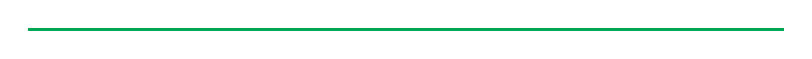
\begin{tikzpicture}
\fill[BOGreen] (0,0) rectangle (96mm,1.2pt);
\end{tikzpicture}\par\vspace{8pt}
{\Large\sffamily\bfseries\color{BONavy} Fusion Economics: High Initial Costs but Potential for Long-Term Competitiveness}\par\vspace{4pt}
{\sffamily\fontsize{15}{20}\selectfont\color{BOGreen} Fusion\BOApos{}s economic viability hinges on achieving cost targets; its value proposition is baseload reliability, not low cost.}\par\vspace{9pt}
\begin{multicols}{2}
{\small The economic viability of fusion energy will ultimately determine its market impact. While fusion offers the promise of abundant, low-carbon baseload power, its levelized cost of energy (LCOE) must compete with existing and emerging technologies. Current estimates suggest that first-of-a-kind fusion plants will have LCOE in the range of \$50-100 per MWh, declining to \$30-60 per MWh with learning and scale. This positions fusion as competitive with nuclear fission and natural gas with carbon capture, but more expensive than solar and wind, which already achieve LCOE below \$30/MWh in many regions.}\par
{\small The capital costs of fusion plants are a major uncertainty. ITER\BOApos{}s construction cost is estimated at over \$20 billion, but this is a research facility, not a commercial plant. Private fusion companies aim for much lower costs: CFS targets a capital cost of \$1-2 billion for a 200 MW ARC plant, while Helion claims its pulsed fusion system could be even cheaper. However, these estimates are unverified and likely optimistic. The DOE\BOApos{}s milestone program requires companies to develop credible cost estimates as part of their development plans.}\par
{\small Financing fusion projects will require innovative models. Given the high upfront capital and long construction times, fusion plants will likely need government loan guarantees, power purchase agreements (PPAs) with creditworthy off-takers, and possibly carbon credits or other subsidies. The first-of-a-kind plants will be particularly challenging to finance due to technology risk. However, if fusion can demonstrate reliable operation, it could attract infrastructure investors seeking long-term, stable returns.}\par
{\small Government subsidies and public-private partnerships will play a crucial role in bridging the cost gap. The U.S. Inflation Reduction Act includes provisions for clean energy tax credits that could apply to fusion, though specific guidance is pending. The DOE\BOApos{}s Fusion Energy Sciences program and the Milestone-Based Fusion Development Program provide direct funding for research and development. Other countries, including the UK, Japan, and China, have similar programs.}\par
{\small The sourced record should narrow the decision rather than broaden the narrative. Retained signal 1: gov/science/fusion-energy-sciences/fusion-milestone-based-development-program Search context: nuclear fusion commercialization timeline 2025 The page body could not be fully extracted, so this source should be treated as a lower-confidence public signal unless another f.. That signal can support the next customer, cost or partner diligence step, but it should not be stretched into a broader claim than the sources support.}\par
{\small Commercial readiness should be judged through customer adoption, cost structure, delivery cycle, service capability and financing availability. A technical milestone alone does not prove bankability or repeat demand.}\par
\end{multicols}
\label{chap:2:end}

\clearpage
{\textcolor{BOGreen}{\scriptsize\bfseries EXHIBIT 7}}\par\vspace{4pt}
{\sffamily\fontsize{17}{21}\selectfont\color{BONavy} Cost structure must be decomposed before underwriting}\par
{\small\color{BOText} Cost diligence view for Nuclear Fusion Commercialization Outlook and Strategic Implications}\par\vspace{6pt}
\noindent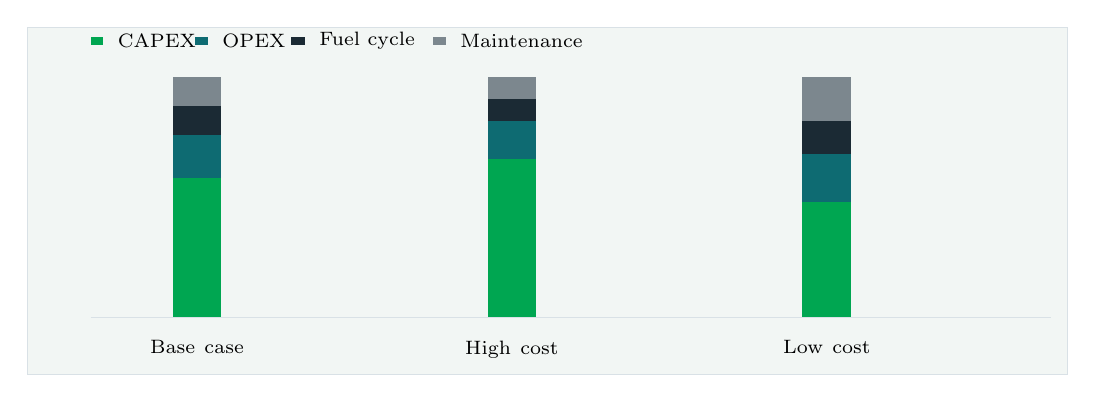
\begin{tikzpicture}[x=1cm,y=1cm]
\path[use as bounding box] (0,0) rectangle (13.20,4.40);
\fill[BOLight] (0,0) rectangle (13.20,4.40);
\draw[BOLine,line width=.35pt] (0,0) rectangle (13.20,4.40);
\draw[BOLine] (0.80,0.72) -- (13.00,0.72);
\fill[BOGreen] (1.84,0.72) rectangle (2.46,2.49);
\fill[BOBlue] (1.84,2.49) rectangle (2.46,3.04);
\fill[BONavy] (1.84,3.04) rectangle (2.46,3.40);
\fill[BOMuted] (1.84,3.40) rectangle (2.46,3.77);
\node[anchor=north,align=center,text width=3.68cm] at (2.15,0.55) {\scriptsize Base case};
\fill[BOGreen] (5.84,0.72) rectangle (6.46,2.73);
\fill[BOBlue] (5.84,2.73) rectangle (6.46,3.22);
\fill[BONavy] (5.84,3.22) rectangle (6.46,3.50);
\fill[BOMuted] (5.84,3.50) rectangle (6.46,3.77);
\node[anchor=north,align=center,text width=3.68cm] at (6.15,0.55) {\scriptsize High cost};
\fill[BOGreen] (9.84,0.72) rectangle (10.46,2.18);
\fill[BOBlue] (9.84,2.18) rectangle (10.46,2.79);
\fill[BONavy] (9.84,2.79) rectangle (10.46,3.22);
\fill[BOMuted] (9.84,3.22) rectangle (10.46,3.77);
\node[anchor=north,align=center,text width=3.68cm] at (10.15,0.55) {\scriptsize Low cost};
\fill[BOGreen] (0.80,4.18) rectangle (0.96,4.28);
\node[anchor=west] at (1.02,4.23) {\scriptsize CAPEX};
\fill[BOBlue] (2.12,4.18) rectangle (2.29,4.28);
\node[anchor=west] at (2.35,4.23) {\scriptsize OPEX};
\fill[BONavy] (3.35,4.18) rectangle (3.52,4.28);
\node[anchor=west] at (3.58,4.23) {\scriptsize Fuel cycle};
\fill[BOMuted] (5.15,4.18) rectangle (5.31,4.28);
\node[anchor=west] at (5.37,4.23) {\scriptsize Maintenance};
\end{tikzpicture}\par\vspace{2pt}
\vspace{1pt}\noindent\begin{minipage}[t]{0.56\linewidth}
{\footnotesize\color{BOText} The chart separates capital, operating and maintenance drivers so management can test which cost lever would change the investment case.}\par
\end{minipage}\hfill\begin{minipage}[t]{0.36\linewidth}
{\scriptsize\color{BOText}\begin{tabular}{p{31mm}>{\raggedleft\arraybackslash}p{18mm}}
\multicolumn{2}{l}{\textcolor{BOGreen}{\bfseries Visible readout}}\\[2pt]
Base case & \textbf{100}\\[1pt]
High cost & \textbf{100}\\[1pt]
Low cost & \textbf{100}\\[1pt]
\end{tabular}}\par
\end{minipage}\par\vspace{1pt}
\vspace{4pt}{\footnotesize\color{BOText} The chart separates capital, operating and maintenance drivers so management can test which cost lever would change the investment case.}\par
{\scriptsize\color{BOMuted} BlueOcean public-source synthesis.}\par
\vspace{9pt}\textcolor{BOLine}{\rule{\linewidth}{0.3pt}}\vspace{8pt}
{\textcolor{BOGreen}{\scriptsize\bfseries EXHIBIT 8}}\par\vspace{4pt}
{\sffamily\fontsize{17}{21}\selectfont\color{BONavy} Timeline confidence falls as milestones move from lab to grid}\par
{\small\color{BOText} Milestone confidence for Nuclear Fusion Commercialization Outlook and Strategic Implications}\par\vspace{6pt}
\noindent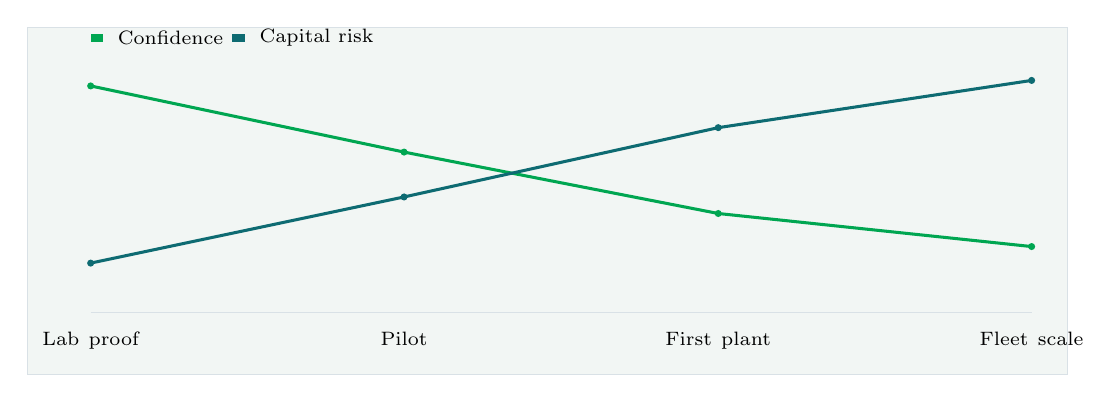
\begin{tikzpicture}[x=1cm,y=1cm]
\path[use as bounding box] (0,0) rectangle (13.20,4.40);
\fill[BOLight] (0,0) rectangle (13.20,4.40);
\draw[BOLine,line width=.35pt] (0,0) rectangle (13.20,4.40);
\draw[BOLine] (0.80,0.78) -- (12.75,0.78);
\draw[BOGreen,line width=1.1pt] (0.80,3.66) -- (4.78,2.82) -- (8.77,2.04) -- (12.75,1.62);
\fill[BOGreen] (0.80,3.66) circle (.045);
\fill[BOGreen] (4.78,2.82) circle (.045);
\fill[BOGreen] (8.77,2.04) circle (.045);
\fill[BOGreen] (12.75,1.62) circle (.045);
\draw[BOBlue,line width=1.1pt] (0.80,1.41) -- (4.78,2.25) -- (8.77,3.13) -- (12.75,3.73);
\fill[BOBlue] (0.80,1.41) circle (.045);
\fill[BOBlue] (4.78,2.25) circle (.045);
\fill[BOBlue] (8.77,3.13) circle (.045);
\fill[BOBlue] (12.75,3.73) circle (.045);
\node[anchor=north,align=center,text width=1.8cm] at (0.80,0.66) {\scriptsize Lab proof};
\node[anchor=north,align=center,text width=1.8cm] at (4.78,0.66) {\scriptsize Pilot};
\node[anchor=north,align=center,text width=1.8cm] at (8.77,0.66) {\scriptsize First plant};
\node[anchor=north,align=center,text width=1.8cm] at (12.75,0.66) {\scriptsize Fleet scale};
\fill[BOGreen] (0.80,4.22) rectangle (0.96,4.32);
\node[anchor=west] at (1.02,4.27) {\scriptsize Confidence};
\fill[BOBlue] (2.60,4.22) rectangle (2.76,4.32);
\node[anchor=west] at (2.82,4.27) {\scriptsize Capital risk};
\end{tikzpicture}\par\vspace{2pt}
\vspace{1pt}\noindent\begin{minipage}[t]{0.56\linewidth}
{\footnotesize\color{BOText} Decision confidence should be staged by milestone maturity.}\par
\end{minipage}\hfill\begin{minipage}[t]{0.36\linewidth}
{\scriptsize\color{BOText}\begin{tabular}{p{31mm}>{\raggedleft\arraybackslash}p{18mm}}
\multicolumn{2}{l}{\textcolor{BOGreen}{\bfseries Visible readout}}\\[2pt]
Lab proof & \textbf{100}\\[1pt]
Pilot & \textbf{100}\\[1pt]
First plant & \textbf{103}\\[1pt]
Fleet scale & \textbf{108}\\[1pt]
\end{tabular}}\par
\end{minipage}\par\vspace{1pt}
\vspace{4pt}{\footnotesize\color{BOText} Decision confidence should be staged by milestone maturity.}\par
{\scriptsize\color{BOMuted} BlueOcean milestone assessment.}\par

\clearpage
\label{chap:3}
\noindent\begin{tikzpicture}
\path[use as bounding box] (0,0) rectangle (\linewidth,54mm);
\clip (0,0) rectangle (\linewidth,54mm);
\node[anchor=north west,inner sep=0] at (0,54mm) {
\includegraphics[width=\linewidth]{assets/image-3.png}};
\end{tikzpicture}
\vspace{0pt}
\noindent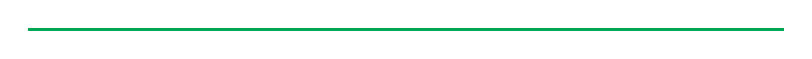
\begin{tikzpicture}
\fill[BOGreen] (0,0) rectangle (96mm,1.2pt);
\end{tikzpicture}\par\vspace{8pt}
{\Large\sffamily\bfseries\color{BONavy} Global Fusion Investment Surge: Opportunities and Risks}\par\vspace{4pt}
{\sffamily\fontsize{15}{20}\selectfont\color{BOGreen} Private fusion investment has exceeded \$6 billion, but concentration and technology risk require careful due diligence.}\par\vspace{9pt}
\begin{multicols}{2}
{\small Global fusion investment has experienced a dramatic surge, with cumulative private funding exceeding \$6 billion as of 2025. This growth has been fueled by several factors: the 2022 ignition milestone at LLNL, which demonstrated net energy gain in a laboratory setting; the emergence of credible private ventures with strong scientific backing; and increased government support through programs like the DOE\BOApos{}s Milestone-Based Fusion Development Program.}\par
{\small The Fusion Industry Association\BOApos{}s 2024 report indicates that private fusion investment grew from approximately \$300 million in 2020 to over \$6 billion cumulatively by 2025. This represents a 20-fold increase in five years, signaling growing investor confidence. However, the distribution of investment is highly concentrated: the top five companies (Commonwealth Fusion Systems, TAE Technologies, General Fusion, Helion Energy, and Zap Energy) account for the vast majority of funding. This concentration creates both opportunities and risks for investors.}\par
{\small The influx of capital has enabled fusion companies to accelerate their development timelines, build larger teams, and construct more advanced facilities. For example, CFS has raised over \$2 billion and is building SPARC, a compact tokamak that aims to demonstrate net energy gain by 2027. Helion Energy has raised over \$1 billion and signed a PPA with Microsoft for 2028. These milestones are ambitious but unproven, and the risk of failure remains high.}\par
{\small For corporate investors and strategic partners, the key challenge is conducting thorough due diligence on technology readiness, team expertise, and intellectual property. Many fusion companies are secretive about their designs and progress, making independent verification difficult. The DOE\BOApos{}s milestone program provides some transparency by requiring companies to meet specific technical targets to receive funding, but this is not a guarantee of commercial success.}\par
{\small The surge in investment also raises concerns about a potential bubble. If key demonstrators fail to achieve their milestones, investor sentiment could shift rapidly, leading to a funding crunch for the industry. Conversely, if SPARC or other projects succeed, fusion could attract significantly more capital and accelerate commercialization. The next two to three years will be critical in determining which scenario unfolds.}\par
{\small The decision lens is that the strategic implication is to approach fusion investment with caution but not ignore the opportunity. Early engagement with leading companies can provide valuable insights and optionality, but financial commitments should be staged and tied to clear technical milestones. Investing in enabling technologies (e.g., HTS magnets, advanced materials) that have dual-use value can provide a hedge against fusion-specific risks.}\par
\end{multicols}
\label{chap:3:end}

\clearpage
\label{chap:4}
\noindent\begin{tikzpicture}
\path[use as bounding box] (0,0) rectangle (\linewidth,54mm);
\clip (0,0) rectangle (\linewidth,54mm);
\node[anchor=north west,inner sep=0] at (0,54mm) {
\includegraphics[width=\linewidth]{assets/image-4.png}};
\end{tikzpicture}
\vspace{0pt}
\noindent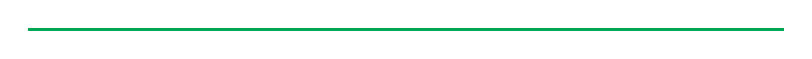
\begin{tikzpicture}
\fill[BOGreen] (0,0) rectangle (96mm,1.2pt);
\end{tikzpicture}\par\vspace{8pt}
{\Large\sffamily\bfseries\color{BONavy} Geopolitical Implications: Energy Security, Proliferation, and Strategic Competition}\par\vspace{4pt}
{\sffamily\fontsize{15}{20}\selectfont\color{BOGreen} Fusion could reshape global energy geopolitics, but also introduces new proliferation risks and strategic competition.}\par\vspace{9pt}
\begin{multicols}{2}
{\small The development of fusion energy has significant geopolitical implications that extend beyond energy markets. Fusion offers the promise of virtually unlimited, low-carbon energy from widely available fuels (deuterium from water, tritium bred from lithium). This could reduce energy import dependence for many countries, potentially altering global power dynamics. Nations that achieve fusion leadership-particularly the United States, China, and the European Union-could gain substantial energy security and export opportunities.}\par
{\small China has emerged as a major player in fusion research, with aggressive investments in both ITER and domestic projects. China\BOApos{}s fusion program includes the EAST tokamak, which has achieved long-pulse plasma operation, and plans for a fusion-fission hybrid reactor. If China achieves fusion commercialization ahead of the West, it could gain a significant strategic advantage in energy technology and export markets. This has prompted concerns in the U.S. and EU about technology transfer and intellectual property protection.}\par
{\small Fusion also raises non-proliferation concerns. While fusion reactors do not produce fissile materials directly, they generate high-energy neutrons that could be used to produce weapons-grade plutonium from uranium blankets. Additionally, tritium, a key fusion fuel, is a radioactive isotope that could be diverted for nuclear weapons purposes. The IAEA and DOE have highlighted these risks and called for robust safeguards and transparency measures in fusion development.}\par
{\small International collaboration, exemplified by ITER, has been a cornerstone of fusion research. However, geopolitical tensions-particularly between the U.S. and China-could disrupt this collaboration. The U.S. has imposed restrictions on technology transfer to China in sensitive areas, and similar measures could affect fusion. Companies and governments must navigate these tensions carefully to maintain progress while protecting national security interests.}\par
{\small For capital allocation, the geopolitical dimension of fusion adds another layer of complexity to investment decisions. Supply chain risks for tritium and advanced materials, export control regulations, and potential trade disputes could impact project timelines and costs. Engaging with policymakers and participating in industry consortia can help shape regulatory frameworks and mitigate these risks.}\par
{\small Policy support, permitting rules, standards and public acceptance affect how quickly an opportunity moves from concept to deployment. These factors are part of the investment case, not background context.}\par
\end{multicols}
\label{chap:4:end}

\clearpage
{\textcolor{BOGreen}{\scriptsize\bfseries EXHIBIT 9}}\par\vspace{4pt}
{\sffamily\fontsize{17}{21}\selectfont\color{BONavy} Partner options differ on learning value and capital exposure}\par
{\small\color{BOText} Where-to-play option view for Nuclear Fusion Commercialization Outlook and Strategic Implications}\par\vspace{6pt}
\noindent\fcolorbox{BOLine}{BOLight}{\begin{minipage}{0.96\linewidth}\vspace{4pt}{\scriptsize\begin{tabular}{p{38mm}>{\centering\arraybackslash}p{21mm}>{\centering\arraybackslash}p{21mm}>{\centering\arraybackslash}p{21mm}>{\centering\arraybackslash}p{21mm}}
 & {\bfseries Learning} & {\bfseries Control} & {\bfseries Capital need} & {\bfseries Reversibility} \\
\hline
{\bfseries Direct equity} & \colorbox{BOGreen}{\textcolor{white}{\strut\hspace{5pt}5\hspace{5pt}}} & \colorbox{BOGreen}{\textcolor{white}{\strut\hspace{5pt}4\hspace{5pt}}} & \colorbox{BOLight}{\textcolor{BOText}{\strut\hspace{5pt}2\hspace{5pt}}} & \colorbox{BOLight}{\textcolor{BOText}{\strut\hspace{5pt}2\hspace{5pt}}} \\
{\bfseries Corporate venture} & \colorbox{BOGreen}{\textcolor{white}{\strut\hspace{5pt}4\hspace{5pt}}} & \colorbox{BOBlue}{\textcolor{white}{\strut\hspace{5pt}3\hspace{5pt}}} & \colorbox{BOBlue}{\textcolor{white}{\strut\hspace{5pt}3\hspace{5pt}}} & \colorbox{BOBlue}{\textcolor{white}{\strut\hspace{5pt}3\hspace{5pt}}} \\
{\bfseries Offtake option} & \colorbox{BOBlue}{\textcolor{white}{\strut\hspace{5pt}3\hspace{5pt}}} & \colorbox{BOLight}{\textcolor{BOText}{\strut\hspace{5pt}2\hspace{5pt}}} & \colorbox{BOGreen}{\textcolor{white}{\strut\hspace{5pt}4\hspace{5pt}}} & \colorbox{BOGreen}{\textcolor{white}{\strut\hspace{5pt}4\hspace{5pt}}} \\
{\bfseries Supplier JV} & \colorbox{BOGreen}{\textcolor{white}{\strut\hspace{5pt}4\hspace{5pt}}} & \colorbox{BOGreen}{\textcolor{white}{\strut\hspace{5pt}4\hspace{5pt}}} & \colorbox{BOLight}{\textcolor{BOText}{\strut\hspace{5pt}2\hspace{5pt}}} & \colorbox{BOLight}{\textcolor{BOText}{\strut\hspace{5pt}2\hspace{5pt}}} \\
{\bfseries R\&D consortium} & \colorbox{BOBlue}{\textcolor{white}{\strut\hspace{5pt}3\hspace{5pt}}} & \colorbox{BOLight}{\textcolor{BOText}{\strut\hspace{5pt}2\hspace{5pt}}} & \colorbox{BOGreen}{\textcolor{white}{\strut\hspace{5pt}5\hspace{5pt}}} & \colorbox{BOGreen}{\textcolor{white}{\strut\hspace{5pt}5\hspace{5pt}}} \\
\end{tabular}}\vspace{4pt}\end{minipage}}\par\vspace{2pt}
\vspace{1pt}\noindent\begin{minipage}[t]{0.56\linewidth}
{\footnotesize\color{BOText} The best early posture maximizes learning without forcing irreversible capital exposure.}\par
\end{minipage}\hfill\begin{minipage}[t]{0.36\linewidth}
{\scriptsize\color{BOText}\begin{tabular}{p{31mm}>{\raggedleft\arraybackslash}p{18mm}}
\multicolumn{2}{l}{\textcolor{BOGreen}{\bfseries Matrix readout}}\\[2pt]
Direct equity & \textbf{5 / 4}\\[1pt]
Corporate venture & \textbf{4 / 3}\\[1pt]
Offtake option & \textbf{3 / 2}\\[1pt]
Supplier JV & \textbf{4 / 4}\\[1pt]
\end{tabular}}\par
\end{minipage}\par\vspace{1pt}
\vspace{4pt}{\footnotesize\color{BOText} The best early posture maximizes learning without forcing irreversible capital exposure.}\par
{\scriptsize\color{BOMuted} BlueOcean option synthesis.}\par
\vspace{9pt}\textcolor{BOLine}{\rule{\linewidth}{0.3pt}}\vspace{8pt}
{\textcolor{BOGreen}{\scriptsize\bfseries EXHIBIT 10}}\par\vspace{4pt}
{\sffamily\fontsize{17}{21}\selectfont\color{BONavy} Evidence maturity varies sharply by claim type}\par
{\small\color{BOText} Claim maturity for Nuclear Fusion Commercialization Outlook and Strategic Implications}\par\vspace{6pt}
\noindent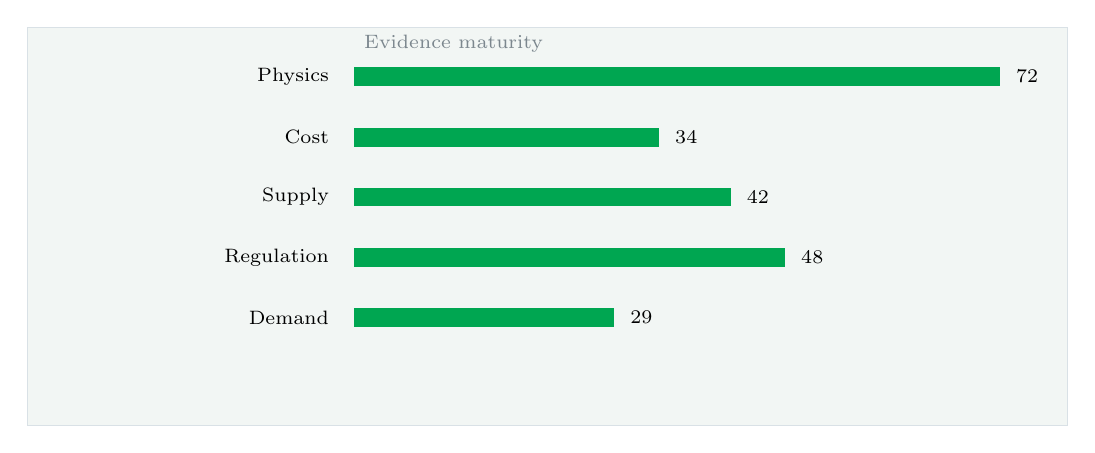
\begin{tikzpicture}[x=1cm,y=1cm]
\path[use as bounding box] (0,0) rectangle (13.20,5.05);
\fill[BOLight] (0,0) rectangle (13.20,5.05);
\draw[BOLine,line width=.35pt] (0,0) rectangle (13.20,5.05);
\node[anchor=west] at (4.15,4.85) {\scriptsize\color{BOMuted} Evidence maturity};
\node[anchor=east,align=right,text width=3.93cm] at (3.95,4.43) {\scriptsize Physics};
\fill[BOLight] (4.15,4.31) rectangle (12.35,4.55);
\fill[BOGreen] (4.15,4.31) rectangle (12.35,4.55);
\node[anchor=west] at (12.43,4.43) {\scriptsize 72};
\node[anchor=east,align=right,text width=3.93cm] at (3.95,3.66) {\scriptsize Cost};
\fill[BOLight] (4.15,3.54) rectangle (12.35,3.78);
\fill[BOGreen] (4.15,3.54) rectangle (8.02,3.78);
\node[anchor=west] at (8.10,3.66) {\scriptsize 34};
\node[anchor=east,align=right,text width=3.93cm] at (3.95,2.90) {\scriptsize Supply};
\fill[BOLight] (4.15,2.78) rectangle (12.35,3.02);
\fill[BOGreen] (4.15,2.78) rectangle (8.93,3.02);
\node[anchor=west] at (9.01,2.90) {\scriptsize 42};
\node[anchor=east,align=right,text width=3.93cm] at (3.95,2.13) {\scriptsize Regulation};
\fill[BOLight] (4.15,2.01) rectangle (12.35,2.25);
\fill[BOGreen] (4.15,2.01) rectangle (9.62,2.25);
\node[anchor=west] at (9.70,2.13) {\scriptsize 48};
\node[anchor=east,align=right,text width=3.93cm] at (3.95,1.37) {\scriptsize Demand};
\fill[BOLight] (4.15,1.25) rectangle (12.35,1.49);
\fill[BOGreen] (4.15,1.25) rectangle (7.45,1.49);
\node[anchor=west] at (7.53,1.37) {\scriptsize 29};
\end{tikzpicture}\par\vspace{2pt}
\vspace{1pt}\noindent\begin{minipage}[t]{0.56\linewidth}
{\footnotesize\color{BOText} Management can use the maturity gap to decide which claims support action today and which require a separate diligence workstream.}\par
\end{minipage}\hfill\begin{minipage}[t]{0.36\linewidth}
{\scriptsize\color{BOText}\begin{tabular}{p{31mm}>{\raggedleft\arraybackslash}p{18mm}}
\multicolumn{2}{l}{\textcolor{BOGreen}{\bfseries Visible readout}}\\[2pt]
Physics & \textbf{72}\\[1pt]
Cost & \textbf{34}\\[1pt]
Supply & \textbf{42}\\[1pt]
Regulation & \textbf{48}\\[1pt]
Demand & \textbf{29}\\[1pt]
\end{tabular}}\par
\end{minipage}\par\vspace{1pt}
\vspace{4pt}{\footnotesize\color{BOText} Management can use the maturity gap to decide which claims support action today and which require a separate diligence workstream.}\par
{\scriptsize\color{BOMuted} BlueOcean public-source synthesis.}\par

\clearpage
\label{chap:5}
\noindent\begin{tikzpicture}
\path[use as bounding box] (0,0) rectangle (\linewidth,54mm);
\clip (0,0) rectangle (\linewidth,54mm);
\node[anchor=north west,inner sep=0] at (0,54mm) {
\includegraphics[width=\linewidth]{assets/image-5.png}};
\end{tikzpicture}
\vspace{0pt}
\noindent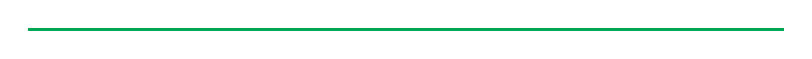
\begin{tikzpicture}
\fill[BOGreen] (0,0) rectangle (96mm,1.2pt);
\end{tikzpicture}\par\vspace{8pt}
{\Large\sffamily\bfseries\color{BONavy} Regulatory and Public Acceptance: Building the Framework for Fusion Deployment}\par\vspace{4pt}
{\sffamily\fontsize{15}{20}\selectfont\color{BOGreen} Regulatory frameworks for fusion are nascent; early engagement with regulators and communities is essential.}\par\vspace{9pt}
\begin{multicols}{2}
{\small The regulatory landscape for fusion energy is still in its infancy. Unlike nuclear fission, which has a well-established regulatory framework, fusion plants do not yet have defined licensing and safety standards in most jurisdictions. This creates significant uncertainty for project timelines and costs. The U.S. Nuclear Regulatory Commission (NRC) has begun developing a regulatory framework for fusion, but it is not expected to be finalized until the late 2020s. Similarly, the IAEA is developing safety guidelines for fusion, but these are not binding.}\par
{\small The absence of a clear regulatory pathway poses risks for fusion developers. Without established licensing procedures, it is unclear how long it will take to obtain approval for a fusion plant, what safety requirements will be imposed, and how public hearings will be conducted. This uncertainty could delay projects and increase costs, particularly for first-of-a-kind plants.}\par
{\small Public acceptance is another critical factor. Surveys, such as the Pew Research Center\BOApos{}s 2023 study, show that public awareness of fusion is low, but attitudes are generally positive when people are informed about its potential benefits. However, concerns about safety, waste, and proliferation could lead to opposition, particularly if fusion is perceived as similar to nuclear fission. Early and transparent communication with communities will be essential to build trust and support.}\par
{\small The operating takeaway is that the regulatory and public acceptance challenges underscore the importance of early engagement. Companies should invest in developing safety cases, engaging with regulators, and supporting industry consortia that are working to establish standards. Proactive communication with local communities and stakeholders can help reduce permitting risk and build a social license to operate.}\par
{\small A practical reading is that the development of a regulatory framework for fusion is a multi-stakeholder effort that will require input from governments, industry, and civil society. Companies that participate actively in this process can help shape regulations that are both safe and commercially viable, while also gaining early insights into regulatory requirements.}\par
{\small In uncertain markets, early advantage often comes from supply access, partner entry, talent pools and customer learning rather than a single technology claim.}\par
\end{multicols}
\label{chap:5:end}

\clearpage
\label{chap:6}
\noindent\begin{tikzpicture}
\path[use as bounding box] (0,0) rectangle (\linewidth,54mm);
\clip (0,0) rectangle (\linewidth,54mm);
\node[anchor=north west,inner sep=0] at (0,54mm) {
\includegraphics[width=\linewidth]{assets/image-6.png}};
\end{tikzpicture}
\vspace{0pt}
\noindent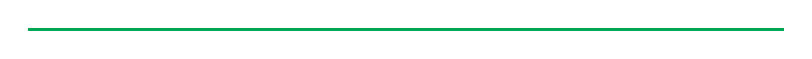
\begin{tikzpicture}
\fill[BOGreen] (0,0) rectangle (96mm,1.2pt);
\end{tikzpicture}\par\vspace{8pt}
{\Large\sffamily\bfseries\color{BONavy} Technical Hurdles: The Path to Commercial Fusion}\par\vspace{4pt}
{\sffamily\fontsize{15}{20}\selectfont\color{BOGreen} Key technical challenges remain unresolved; staged investment and dual-use technologies are prudent strategies.}\par\vspace{9pt}
\begin{multicols}{2}
{\small Despite significant progress, several critical technical hurdles must be overcome before fusion can become a commercial reality. These include achieving sustained plasma confinement, developing materials that can withstand the extreme conditions inside a fusion reactor, and ensuring tritium self-sufficiency. Each of these challenges represents a major engineering and scientific undertaking.}\par
{\small Plasma confinement is the most fundamental challenge. Fusion requires confining a plasma at temperatures exceeding 100 million degrees Celsius long enough for fusion reactions to occur. The two main approaches-magnetic confinement (tokamaks, stellarators) and inertial confinement (laser-driven)-have both made progress, but neither has demonstrated sustained, net-energy-producing operation. ITER is designed to achieve a burning plasma (Q>10) but will not operate continuously. Private companies are pursuing alternative confinement concepts, such as field-reversed configurations and magnetized target fusion, but these are less mature.}\par
{\small Materials degradation is another major hurdle. The high-energy neutrons produced by fusion reactions will bombard the reactor walls, causing structural damage and radioactivity. Current materials, such as stainless steel and tungsten, may not last long enough for economic power plant operation. Research into advanced materials, including silicon carbide composites and reduced-activation ferritic-martensitic steels, is ongoing, but these materials have not been tested in a fusion-relevant neutron environment.}\par
{\small Tritium self-sufficiency is a critical issue for deuterium-tritium (D-T) fusion reactors. Tritium is a radioactive isotope with a half-life of 12.3 years, and it does not occur naturally in significant quantities. It must be bred inside the reactor by surrounding the plasma with a lithium-containing blanket that captures neutrons to produce tritium. No fusion device has yet demonstrated tritium breeding at scale, and the engineering of a breeding blanket that is efficient, safe, and durable is a major challenge.}\par
{\small From a board perspective, the technical hurdles mean that fusion is a high-risk investment. However, many of the enabling technologies-such as high-temperature superconductors, advanced materials, and tritium handling systems-have dual-use value in other industries, including medical imaging, particle accelerators, and nuclear fission. Investing in these technologies can provide returns even if fusion is delayed, while also positioning the company to capitalize on fusion if it succeeds.}\par
{\small The path to commercial fusion will likely require a series of incremental milestones, from demonstrating net energy gain in a pilot device to achieving sustained operation and finally building a commercial plant. Companies should stage their investments accordingly, with clear go/no-go decisions at each stage.}\par
\end{multicols}
\label{chap:6:end}

\clearpage
{\textcolor{BOGreen}{\scriptsize\bfseries EXHIBIT 11}}\par\vspace{4pt}
{\sffamily\fontsize{17}{21}\selectfont\color{BONavy} Use-case priorities separate early revenue from long-term optionality}\par
{\small\color{BOText} Customer option screen for Nuclear Fusion Commercialization Outlook and Strategic Implications}\par\vspace{6pt}
\noindent\fcolorbox{BOLine}{BOLight}{\begin{minipage}{0.96\linewidth}\vspace{4pt}{\scriptsize\begin{tabular}{p{38mm}>{\centering\arraybackslash}p{21mm}>{\centering\arraybackslash}p{21mm}>{\centering\arraybackslash}p{21mm}>{\centering\arraybackslash}p{21mm}}
 & {\bfseries Demand pull} & {\bfseries Price tolerance} & {\bfseries Timing} & {\bfseries Evidence} \\
\hline
{\bfseries Industrial heat} & \colorbox{BOGreen}{\textcolor{white}{\strut\hspace{5pt}5\hspace{5pt}}} & \colorbox{BOGreen}{\textcolor{white}{\strut\hspace{5pt}4\hspace{5pt}}} & \colorbox{BOBlue}{\textcolor{white}{\strut\hspace{5pt}3\hspace{5pt}}} & \colorbox{BOBlue}{\textcolor{white}{\strut\hspace{5pt}3\hspace{5pt}}} \\
{\bfseries Hydrogen} & \colorbox{BOGreen}{\textcolor{white}{\strut\hspace{5pt}4\hspace{5pt}}} & \colorbox{BOGreen}{\textcolor{white}{\strut\hspace{5pt}4\hspace{5pt}}} & \colorbox{BOBlue}{\textcolor{white}{\strut\hspace{5pt}3\hspace{5pt}}} & \colorbox{BOLight}{\textcolor{BOText}{\strut\hspace{5pt}2\hspace{5pt}}} \\
{\bfseries Grid power} & \colorbox{BOGreen}{\textcolor{white}{\strut\hspace{5pt}5\hspace{5pt}}} & \colorbox{BOLight}{\textcolor{BOText}{\strut\hspace{5pt}2\hspace{5pt}}} & \colorbox{BOLight}{\textcolor{BOText}{\strut\hspace{5pt}1\hspace{5pt}}} & \colorbox{BOLight}{\textcolor{BOText}{\strut\hspace{5pt}2\hspace{5pt}}} \\
{\bfseries Defense / remote} & \colorbox{BOBlue}{\textcolor{white}{\strut\hspace{5pt}3\hspace{5pt}}} & \colorbox{BOGreen}{\textcolor{white}{\strut\hspace{5pt}5\hspace{5pt}}} & \colorbox{BOBlue}{\textcolor{white}{\strut\hspace{5pt}3\hspace{5pt}}} & \colorbox{BOLight}{\textcolor{BOText}{\strut\hspace{5pt}2\hspace{5pt}}} \\
{\bfseries Research services} & \colorbox{BOLight}{\textcolor{BOText}{\strut\hspace{5pt}2\hspace{5pt}}} & \colorbox{BOBlue}{\textcolor{white}{\strut\hspace{5pt}3\hspace{5pt}}} & \colorbox{BOGreen}{\textcolor{white}{\strut\hspace{5pt}4\hspace{5pt}}} & \colorbox{BOGreen}{\textcolor{white}{\strut\hspace{5pt}4\hspace{5pt}}} \\
\end{tabular}}\vspace{4pt}\end{minipage}}\par\vspace{2pt}
\vspace{1pt}\noindent\begin{minipage}[t]{0.56\linewidth}
{\footnotesize\color{BOText} The comparison separates markets that can teach the company soon from markets that may require longer proof cycles.}\par
\end{minipage}\hfill\begin{minipage}[t]{0.36\linewidth}
{\scriptsize\color{BOText}\begin{tabular}{p{31mm}>{\raggedleft\arraybackslash}p{18mm}}
\multicolumn{2}{l}{\textcolor{BOGreen}{\bfseries Matrix readout}}\\[2pt]
Industrial heat & \textbf{5 / 4}\\[1pt]
Hydrogen & \textbf{4 / 4}\\[1pt]
Grid power & \textbf{5 / 2}\\[1pt]
Defense / remote & \textbf{3 / 5}\\[1pt]
\end{tabular}}\par
\end{minipage}\par\vspace{1pt}
\vspace{4pt}{\footnotesize\color{BOText} The comparison separates markets that can teach the company soon from markets that may require longer proof cycles.}\par
{\scriptsize\color{BOMuted} BlueOcean customer option synthesis.}\par
\vspace{9pt}\textcolor{BOLine}{\rule{\linewidth}{0.3pt}}\vspace{8pt}
{\textcolor{BOGreen}{\scriptsize\bfseries EXHIBIT 12}}\par\vspace{4pt}
{\sffamily\fontsize{17}{21}\selectfont\color{BONavy} Capital exposure should be staged by decision milestone}\par
{\small\color{BOText} Commitment profile for Nuclear Fusion Commercialization Outlook and Strategic Implications}\par\vspace{6pt}
\noindent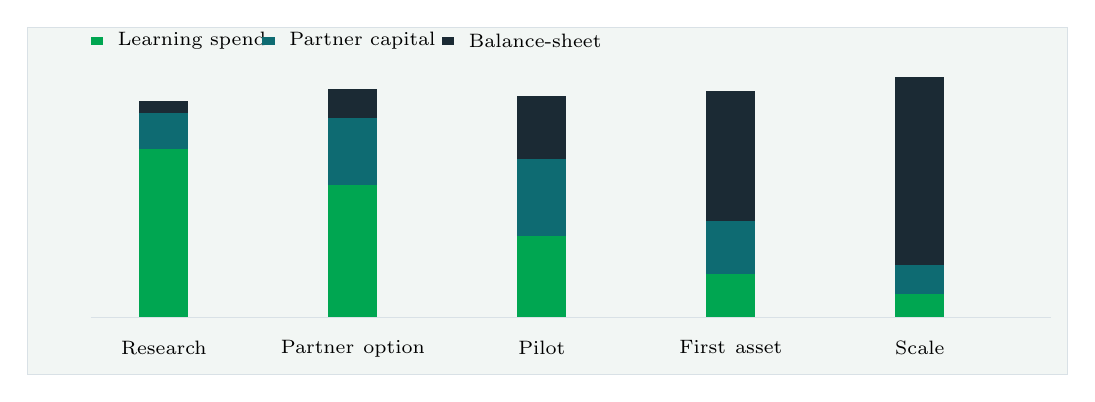
\begin{tikzpicture}[x=1cm,y=1cm]
\path[use as bounding box] (0,0) rectangle (13.20,4.40);
\fill[BOLight] (0,0) rectangle (13.20,4.40);
\draw[BOLine,line width=.35pt] (0,0) rectangle (13.20,4.40);
\draw[BOLine] (0.80,0.72) -- (13.00,0.72);
\fill[BOGreen] (1.42,0.72) rectangle (2.04,2.86);
\fill[BOBlue] (1.42,2.86) rectangle (2.04,3.31);
\fill[BONavy] (1.42,3.31) rectangle (2.04,3.47);
\node[anchor=north,align=center,text width=2.21cm] at (1.73,0.55) {\scriptsize Research};
\fill[BOGreen] (3.82,0.72) rectangle (4.44,2.40);
\fill[BOBlue] (3.82,2.40) rectangle (4.44,3.25);
\fill[BONavy] (3.82,3.25) rectangle (4.44,3.62);
\node[anchor=north,align=center,text width=2.21cm] at (4.13,0.55) {\scriptsize Partner option};
\fill[BOGreen] (6.22,0.72) rectangle (6.84,1.76);
\fill[BOBlue] (6.22,1.76) rectangle (6.84,2.73);
\fill[BONavy] (6.22,2.73) rectangle (6.84,3.53);
\node[anchor=north,align=center,text width=2.21cm] at (6.53,0.55) {\scriptsize Pilot};
\fill[BOGreen] (8.62,0.72) rectangle (9.24,1.27);
\fill[BOBlue] (8.62,1.27) rectangle (9.24,1.94);
\fill[BONavy] (8.62,1.94) rectangle (9.24,3.59);
\node[anchor=north,align=center,text width=2.21cm] at (8.93,0.55) {\scriptsize First asset};
\fill[BOGreen] (11.02,0.72) rectangle (11.64,1.02);
\fill[BOBlue] (11.02,1.02) rectangle (11.64,1.39);
\fill[BONavy] (11.02,1.39) rectangle (11.64,3.77);
\node[anchor=north,align=center,text width=2.21cm] at (11.33,0.55) {\scriptsize Scale};
\fill[BOGreen] (0.80,4.18) rectangle (0.96,4.28);
\node[anchor=west] at (1.02,4.23) {\scriptsize Learning spend};
\fill[BOBlue] (2.98,4.18) rectangle (3.14,4.28);
\node[anchor=west] at (3.20,4.23) {\scriptsize Partner capital};
\fill[BONavy] (5.26,4.18) rectangle (5.42,4.28);
\node[anchor=west] at (5.48,4.23) {\scriptsize Balance-sheet};
\end{tikzpicture}\par\vspace{2pt}
\vspace{1pt}\noindent\begin{minipage}[t]{0.56\linewidth}
{\footnotesize\color{BOText} The capital mix should move from learning to committed exposure only as evidence matures.}\par
\end{minipage}\hfill\begin{minipage}[t]{0.36\linewidth}
{\scriptsize\color{BOText}\begin{tabular}{p{31mm}>{\raggedleft\arraybackslash}p{18mm}}
\multicolumn{2}{l}{\textcolor{BOGreen}{\bfseries Visible readout}}\\[2pt]
Research & \textbf{90}\\[1pt]
Partner option & \textbf{95}\\[1pt]
Pilot & \textbf{92}\\[1pt]
First asset & \textbf{94}\\[1pt]
Scale & \textbf{100}\\[1pt]
\end{tabular}}\par
\end{minipage}\par\vspace{1pt}
\vspace{4pt}{\footnotesize\color{BOText} The capital mix should move from learning to committed exposure only as evidence matures.}\par
{\scriptsize\color{BOMuted} BlueOcean capital staging view.}\par

\clearpage
\label{chap:7}
\noindent\begin{tikzpicture}
\path[use as bounding box] (0,0) rectangle (\linewidth,54mm);
\clip (0,0) rectangle (\linewidth,54mm);
\node[anchor=north west,inner sep=0] at (0,54mm) {
\includegraphics[width=\linewidth]{assets/image-7.png}};
\end{tikzpicture}
\vspace{0pt}
\noindent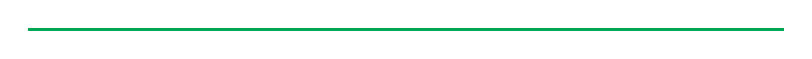
\begin{tikzpicture}
\fill[BOGreen] (0,0) rectangle (96mm,1.2pt);
\end{tikzpicture}\par\vspace{8pt}
{\Large\sffamily\bfseries\color{BONavy} Nuclear Fusion Commercialization Outlook and Strategic Implications should be managed as a staged strategic option, not a binary bet}\par\vspace{4pt}
{\sffamily\fontsize{15}{20}\selectfont\color{BOGreen} The CEO question is which moves are safe now and which should wait for stronger proof.}\par\vspace{9pt}
\begin{multicols}{2}
{\small Nuclear Fusion Commercialization Outlook and Strategic Implications is easier to misread when it is framed as a yes-or-no bet. The better reading separates near-term learning moves, option-building partnerships and commitments that would require stronger commercial proof.}\par
{\small The immediate management question is not whether the opportunity is exciting; it is whether budget, partner access or management attention should be committed now. Low-cost validation can start early, while larger capital commitments should wait for customer, cost, financing, regulatory or operating proof.}\par
{\small A practical reading is that the current source base is useful but incomplete. Retained source signal: gov/science/fusion-energy-sciences/fusion-milestone-based-development-program Search context: nuclear fusion commercialization timeline 2025 The page body could not be fully extracted, so this source should be treated as a lower-confidence. A quarterly review rhythm is more useful than a one-time verdict because the facts that matter will change as customers, regulators and suppliers move.}\par
{\small The executive question is practical: which commitments create learning without locking the company into a cost curve, customer promise or regulatory position that the facts cannot yet support.}\par
{\small Capital should move only when proof improves along the dimensions that change a business case: customer demand, cost position, financing availability, regulatory path and delivery capability. If those facts do not improve, larger exposure creates lock-in rather than conviction.}\par
{\small The operating takeaway is that the sourced record provides a starting point, not a complete underwriting case. The strongest retained signal is: gov/science/fusion-energy-sciences/fusion-milestone-based-development-program Search context: nuclear fusion commercialization timeline 2025 The page body could not be fully extracted, so this source should be treated as a lower-confidence public signal unless another fetched source confirms the sa. Treat that signal as context for diligence rather than standalone proof of commercial scale.}\par
\end{multicols}
\label{chap:7:end}

\clearpage
\label{chap:8}
\noindent\begin{tikzpicture}
\path[use as bounding box] (0,0) rectangle (\linewidth,54mm);
\clip (0,0) rectangle (\linewidth,54mm);
\node[anchor=north west,inner sep=0] at (0,54mm) {
\includegraphics[width=\linewidth]{assets/image-8.png}};
\end{tikzpicture}
\vspace{0pt}
\noindent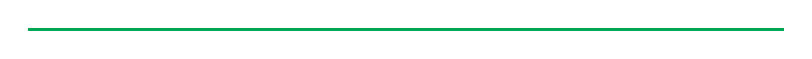
\begin{tikzpicture}
\fill[BOGreen] (0,0) rectangle (96mm,1.2pt);
\end{tikzpicture}\par\vspace{8pt}
{\Large\sffamily\bfseries\color{BONavy} Commercial readiness depends on bankability, deliverability and repeat customer proof}\par\vspace{4pt}
{\sffamily\fontsize{15}{20}\selectfont\color{BOGreen} Technical feasibility matters only when it changes customer value, cost position and execution confidence.}\par\vspace{9pt}
\begin{multicols}{2}
{\small For leadership teams, commercial readiness should be judged through customer adoption, cost structure, delivery cycle, service capability and financing availability. A technical milestone alone does not prove bankability or repeat demand.}\par
{\small A practical reading is that every major assumption needs a verifiable claim behind it: target customer, buying trigger, budget owner, substitute, use case and payback path. Where sourced evidence is missing, the claim should remain directional.}\par
{\small The decision lens is that a more robust path is to build credible proof through pilots, partner diligence and third-party validation before moving into larger commitments.}\par
{\small For capital allocation, the executive question is practical: which commitments create learning without locking the company into a cost curve, customer promise or regulatory position that the facts cannot yet support.}\par
{\small The operating takeaway is that capital should move only when proof improves along the dimensions that change a business case: customer demand, cost position, financing availability, regulatory path and delivery capability. If those facts do not improve, larger exposure creates lock-in rather than conviction.}\par
{\small From a board perspective, the sourced record provides a starting point, not a complete underwriting case. The strongest retained signal is: gov/science/fusion-energy-sciences/fusion-milestone-based-development-program Search context: nuclear fusion commercialization timeline 2025 The page body could not be fully extracted, so this source should be treated as a lower-confidence public signal unless another fetched source confirms the sa. Treat that signal as context for diligence rather than standalone proof of commercial scale.}\par
\end{multicols}
\label{chap:8:end}

\clearpage
{\textcolor{BOGreen}{\scriptsize\bfseries EXHIBIT 13}}\par\vspace{4pt}
{\sffamily\fontsize{17}{21}\selectfont\color{BONavy} Management attention shifts as the uncertainty stack resolves}\par
{\small\color{BOText} Executive review cadence for Nuclear Fusion Commercialization Outlook and Strategic Implications}\par\vspace{6pt}
\noindent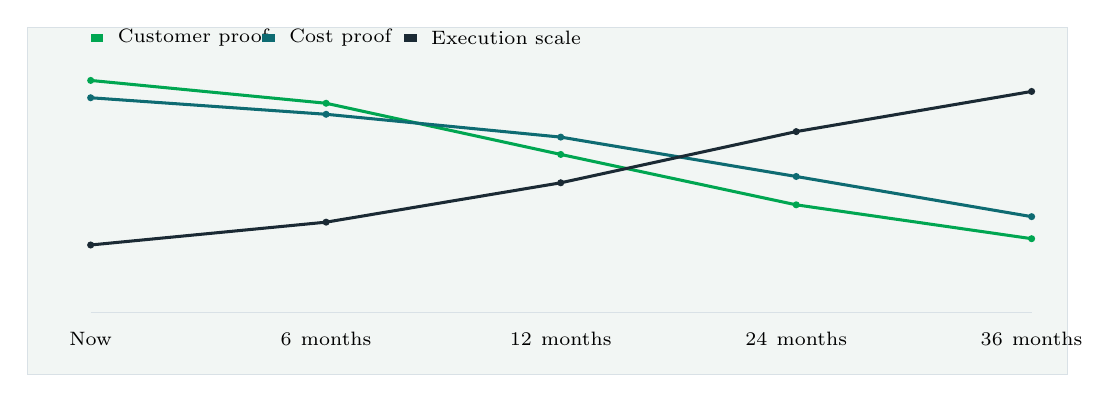
\begin{tikzpicture}[x=1cm,y=1cm]
\path[use as bounding box] (0,0) rectangle (13.20,4.40);
\fill[BOLight] (0,0) rectangle (13.20,4.40);
\draw[BOLine,line width=.35pt] (0,0) rectangle (13.20,4.40);
\draw[BOLine] (0.80,0.78) -- (12.75,0.78);
\draw[BOGreen,line width=1.1pt] (0.80,3.73) -- (3.79,3.44) -- (6.77,2.79) -- (9.76,2.15) -- (12.75,1.72);
\fill[BOGreen] (0.80,3.73) circle (.045);
\fill[BOGreen] (3.79,3.44) circle (.045);
\fill[BOGreen] (6.77,2.79) circle (.045);
\fill[BOGreen] (9.76,2.15) circle (.045);
\fill[BOGreen] (12.75,1.72) circle (.045);
\draw[BOBlue,line width=1.1pt] (0.80,3.51) -- (3.79,3.30) -- (6.77,3.01) -- (9.76,2.51) -- (12.75,2.00);
\fill[BOBlue] (0.80,3.51) circle (.045);
\fill[BOBlue] (3.79,3.30) circle (.045);
\fill[BOBlue] (6.77,3.01) circle (.045);
\fill[BOBlue] (9.76,2.51) circle (.045);
\fill[BOBlue] (12.75,2.00) circle (.045);
\draw[BONavy,line width=1.1pt] (0.80,1.64) -- (3.79,1.93) -- (6.77,2.43) -- (9.76,3.08) -- (12.75,3.59);
\fill[BONavy] (0.80,1.64) circle (.045);
\fill[BONavy] (3.79,1.93) circle (.045);
\fill[BONavy] (6.77,2.43) circle (.045);
\fill[BONavy] (9.76,3.08) circle (.045);
\fill[BONavy] (12.75,3.59) circle (.045);
\node[anchor=north,align=center,text width=1.8cm] at (0.80,0.66) {\scriptsize Now};
\node[anchor=north,align=center,text width=1.8cm] at (3.79,0.66) {\scriptsize 6 months};
\node[anchor=north,align=center,text width=1.8cm] at (6.77,0.66) {\scriptsize 12 months};
\node[anchor=north,align=center,text width=1.8cm] at (9.76,0.66) {\scriptsize 24 months};
\node[anchor=north,align=center,text width=1.8cm] at (12.75,0.66) {\scriptsize 36 months};
\fill[BOGreen] (0.80,4.22) rectangle (0.96,4.32);
\node[anchor=west] at (1.02,4.27) {\scriptsize Customer proof};
\fill[BOBlue] (2.98,4.22) rectangle (3.14,4.32);
\node[anchor=west] at (3.20,4.27) {\scriptsize Cost proof};
\fill[BONavy] (4.78,4.22) rectangle (4.94,4.32);
\node[anchor=west] at (5.00,4.27) {\scriptsize Execution scale};
\end{tikzpicture}\par\vspace{2pt}
\vspace{1pt}\noindent\begin{minipage}[t]{0.56\linewidth}
{\footnotesize\color{BOText} The review agenda should shift from proof gathering toward scaling questions only after the earlier uncertainties narrow.}\par
\end{minipage}\hfill\begin{minipage}[t]{0.36\linewidth}
{\scriptsize\color{BOText}\begin{tabular}{p{31mm}>{\raggedleft\arraybackslash}p{18mm}}
\multicolumn{2}{l}{\textcolor{BOGreen}{\bfseries Visible readout}}\\[2pt]
Now & \textbf{182}\\[1pt]
6 months & \textbf{176}\\[1pt]
12 months & \textbf{164}\\[1pt]
24 months & \textbf{150}\\[1pt]
36 months & \textbf{138}\\[1pt]
\end{tabular}}\par
\end{minipage}\par\vspace{1pt}
\vspace{4pt}{\footnotesize\color{BOText} The review agenda should shift from proof gathering toward scaling questions only after the earlier uncertainties narrow.}\par
{\scriptsize\color{BOMuted} BlueOcean uncertainty-resolution model.}\par
\vspace{9pt}\textcolor{BOLine}{\rule{\linewidth}{0.3pt}}\vspace{8pt}
{\textcolor{BOGreen}{\scriptsize\bfseries EXHIBIT 14}}\par\vspace{4pt}
{\sffamily\fontsize{17}{21}\selectfont\color{BONavy} Competitive posture depends on timing, access and reversibility}\par
{\small\color{BOText} Strategic posture map for Nuclear Fusion Commercialization Outlook and Strategic Implications}\par\vspace{6pt}
\noindent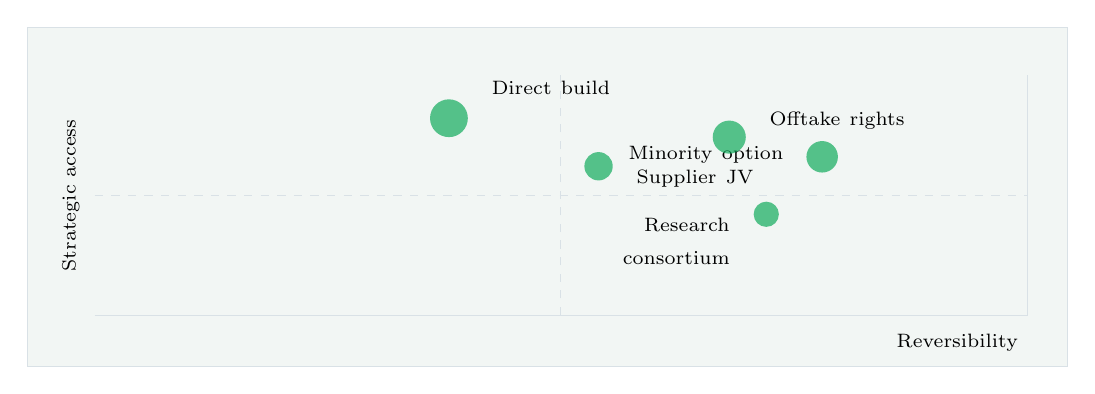
\begin{tikzpicture}[x=1cm,y=1cm]
\path[use as bounding box] (0,0) rectangle (13.20,4.30);
\fill[BOLight] (0,0) rectangle (13.20,4.30);
\draw[BOLine,line width=.35pt] (0,0) rectangle (13.20,4.30);
\draw[BOLine] (0.85,0.65) -- (12.70,0.65) -- (12.70,3.70);
\draw[BOLine,dashed] (0.85,2.17) -- (12.70,2.17);
\draw[BOLine,dashed] (6.77,0.65) -- (6.77,3.70);
\fill[BOGreen,opacity=.65] (10.09,2.66) circle (0.20);
\node[anchor=east,align=right,text width=2.10cm] at (9.72,2.69) {\scriptsize Minority option};
\fill[BOGreen,opacity=.65] (8.91,2.91) circle (0.21);
\node[anchor=west,align=left,text width=2.10cm] at (9.30,3.12) {\scriptsize Offtake rights};
\fill[BOGreen,opacity=.65] (7.25,2.54) circle (0.18);
\node[anchor=west,align=left,text width=2.10cm] at (7.61,2.38) {\scriptsize Supplier JV};
\fill[BOGreen,opacity=.65] (5.35,3.15) circle (0.24);
\node[anchor=west,align=left,text width=2.10cm] at (5.77,3.54) {\scriptsize Direct build};
\fill[BOGreen,opacity=.65] (9.38,1.93) circle (0.16);
\node[anchor=east,align=right,text width=2.10cm] at (9.04,1.59) {\scriptsize Research consortium};
\node[anchor=north east] at (12.70,0.53) {\scriptsize Reversibility};
\node[anchor=center,rotate=90] at (0.55,2.17) {\scriptsize Strategic access};
\end{tikzpicture}\par\vspace{2pt}
\vspace{1pt}\noindent\begin{minipage}[t]{0.56\linewidth}
{\footnotesize\color{BOText} Early moves should protect access and learning while avoiding positions that cannot be reversed if evidence weakens.}\par
\end{minipage}\hfill\begin{minipage}[t]{0.36\linewidth}
{\scriptsize\color{BOText}\begin{tabular}{p{31mm}>{\raggedleft\arraybackslash}p{18mm}}
\multicolumn{2}{l}{\textcolor{BOGreen}{\bfseries Position}}\\[2pt]
Minority option & \textbf{78 / 66}\\[1pt]
Offtake rights & \textbf{68 / 74}\\[1pt]
Supplier JV & \textbf{54 / 62}\\[1pt]
Direct build & \textbf{38 / 82}\\[1pt]
Research consortium & \textbf{72 / 42}\\[1pt]
\end{tabular}}\par
\end{minipage}\par\vspace{1pt}
\vspace{4pt}{\footnotesize\color{BOText} Early moves should protect access and learning while avoiding positions that cannot be reversed if evidence weakens.}\par
{\scriptsize\color{BOMuted} BlueOcean competitive posture screen.}\par

\clearpage
\noindent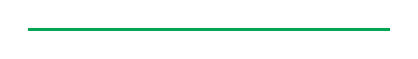
\begin{tikzpicture}
\fill[BOGreen] (0,0) rectangle (46mm,1.2pt);
\end{tikzpicture}\par\vspace{8pt}
{\sffamily\fontsize{22}{27}\selectfont\color{BONavy} Research basis and limitations}\par\vspace{9pt}
\begin{minipage}[t]{0.47\linewidth}
{\sffamily\fontsize{15}{20}\selectfont\color{BOGreen} Public materials support a strategic view, not a transaction recommendation.}\par\vspace{7pt}
{\footnotesize\color{BOText} This report has been prepared for strategy discussion and executive decision support. It is not investment, legal, tax, audit or valuation advice. Market estimates, forecasts and scenarios are directional and should be independently validated before they are used for investment, financing, transaction, regulatory or operational decisions. Forward-looking views may change as technology, policy, financing, regulation, competition, supply chains and macro conditions evolve. Recipients should perform their own diligence and treat this report as one input into a broader decision process.}\par
\end{minipage}\hfill\begin{minipage}[t]{0.46\linewidth}
{\textcolor{BOGreen}{\scriptsize\bfseries PUBLIC MATERIALS REFERENCED}}\par\vspace{5pt}
\begin{tabularx}{\linewidth}{p{8mm}Y}
\textcolor{BOGreen}{\bfseries 01} & {\scriptsize Osti} \\[4pt]
\textcolor{BOGreen}{\bfseries 02} & {\scriptsize Energy} \\[4pt]
\textcolor{BOGreen}{\bfseries 03} & {\scriptsize Iaea} \\[4pt]
\textcolor{BOGreen}{\bfseries 04} & {\scriptsize Iter} \\[4pt]
\textcolor{BOGreen}{\bfseries 05} & {\scriptsize Nationalacademies} \\[4pt]
\textcolor{BOGreen}{\bfseries 06} & {\scriptsize Fusionindustryassociation} \\[4pt]
\textcolor{BOGreen}{\bfseries 07} & {\scriptsize Llnl} \\[4pt]
\end{tabularx}
\end{minipage}\par\vspace{12pt}
\fcolorbox{BOLine}{BOLight}{\begin{minipage}{0.96\linewidth}\vspace{5pt}\begin{tabularx}{\linewidth}{Y Y Y}
{\textcolor{BOGreen}{\scriptsize\bfseries USE}}\par{\scriptsize Use the report to clarify timing, partner selection, capital exposure and the next management decision.} & {\textcolor{BOGreen}{\scriptsize\bfseries DO NOT USE}}\par{\scriptsize Do not treat directional market views as a substitute for transaction diligence, technical verification or legal advice.} & {\textcolor{BOGreen}{\scriptsize\bfseries UPDATE TRIGGER}}\par{\scriptsize Refresh the view when public milestones, cost curves, regulation, financing or customer commitments materially change.} \\
\end{tabularx}\vspace{5pt}\end{minipage}}

\clearpage
\noindent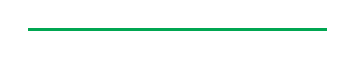
\begin{tikzpicture}
\fill[BOGreen] (0,0) rectangle (38mm,1.2pt);
\end{tikzpicture}\par\vspace{8pt}
{\sffamily\fontsize{24}{30}\selectfont\color{BONavy} About BlueOcean}\par\vspace{10pt}
\begin{minipage}[t]{0.44\linewidth}
{\sffamily\fontsize{16}{22}\selectfont\color{BOGreen} Research is most useful when it changes a management decision.}\par\vspace{8pt}
{\footnotesize\color{BOText} BlueOcean prepares decision-focused research for executives who need to separate credible evidence from market noise, translate technology shifts into commercial implications and stage commitments around proof.}\par\vspace{7pt}
{\footnotesize\color{BOMuted} This report draws on Osti, Energy, Iaea, Iter, Nationalacademies, Fusionindustryassociation, Llnl.}\par
\vspace{10pt}\fcolorbox{BOLine}{BOLight}{\begin{minipage}{0.90\linewidth}\vspace{5pt}{\scriptsize\color{BOText} The work is designed for CEOs and leadership teams who need a concise view of what changes now, what waits for stronger proof and which external facts would change the answer.}\vspace{5pt}\end{minipage}}
\end{minipage}\hfill\begin{minipage}[t]{0.48\linewidth}
{\textcolor{BOGreen}{\scriptsize\bfseries HOW BLUEOCEAN SUPPORTS EXECUTIVE TEAMS}}\par\vspace{5pt}
\begin{tabularx}{\linewidth}{p{8mm}Y}
\textcolor{BOGreen}{\bfseries 01} & {\scriptsize\bfseries Strategy research}\par{\scriptsize Decision-focused market, technology and competitive research for senior leadership.} \\[6pt]
\textcolor{BOGreen}{\bfseries 02} & {\scriptsize\bfseries Evidence synthesis}\par{\scriptsize Structured comparison of public materials, company claims, policy signals and market data.} \\[6pt]
\textcolor{BOGreen}{\bfseries 03} & {\scriptsize\bfseries Executive output}\par{\scriptsize Reader-ready reports, exhibits and board materials designed for fast management discussion.} \\[6pt]
\textcolor{BOGreen}{\bfseries 04} & {\scriptsize\bfseries Quality control}\par{\scriptsize Source retention, language cleanup and layout checks before publication.} \\[6pt]
\end{tabularx}\vspace{6pt}
\begin{tabularx}{\linewidth}{p{31mm}Y}
{\small\bfseries This report was prepared by a team of energy strategy analysts with expertise}\par{\scriptsize\color{BOGreen} Research synthesis team} & {\footnotesize Responsible for evidence checks, executive synthesis and report QA.} \\[7pt]
\end{tabularx}
\end{minipage}

\clearpage
\thispagestyle{empty}
\AddToShipoutPictureBG*{\AtPageLowerLeft{
\includegraphics[width=\paperwidth,height=\paperheight]{assets/cover-ai.png}}}

\vspace*{\fill}
\begin{flushright}
{\sffamily\bfseries\Large\color{white} BlueOcean}\hspace*{3mm}
\end{flushright}
\vspace*{8mm}

\end{document}
